\documentclass{article}

% SOURCE_DATE_EPOCH fixes the PDF dates in the build environment. Suppress the
% otherwise implementation-dependent trailer ID and pdfTeX provenance records.
\ifdefined\pdftrailerid
  \pdftrailerid{}
\fi
\ifdefined\pdfsuppressptexinfo
  \pdfsuppressptexinfo=-1
\fi

\PassOptionsToPackage{numbers, compress}{natbib}
\usepackage[final,main]{neurips_2026}

\usepackage[utf8]{inputenc}
\usepackage[T1]{fontenc}
\usepackage{hyperref}
\usepackage{url}
\usepackage{booktabs}
\usepackage{amsfonts}
\usepackage{amsmath}
\usepackage{amssymb}
\usepackage{amsthm}
\usepackage{nicefrac}
\usepackage{microtype}
\usepackage{xcolor}
\usepackage{graphicx}
\usepackage{subcaption}
\usepackage{algorithm}
\usepackage{algpseudocode}
\usepackage{wrapfig}
\usepackage{multirow}

\DeclareMathOperator*{\argmin}{arg\,min}
\DeclareMathOperator{\minSR}{minSR}
\newcommand{\Expect}{\mathbb{E}}
\newcommand{\Real}{\mathbb{R}}
\newcommand{\Snorm}[1]{\left\| #1 \right\|_S^2}

\title{Stochastic Reconfiguration as Statistical Filtering for Overparameterized Neural Quantum States}

\author{%
  Tak Hur \\
  Department of Statistics and Data Science \\
  Yonsei University \\
  Seoul, Republic of Korea \\
  \texttt{takh0404@yonsei.ac.kr} \\
}

\hypersetup{
  pdftitle={Stochastic Reconfiguration as Statistical Filtering for Overparameterized Neural Quantum States},
  pdfauthor={Tak Hur}
}
  
\begin{document}

\maketitle

\begin{abstract}
Stochastic reconfiguration (SR) is the standard optimizer for neural quantum
states (NQS), but modern NQS often have far more parameters than Monte Carlo
samples. We show that in this regime the diagonal shift is more than a numerical
stabilizer. It acts as a statistical filter for finite-sample generalization.
At a fixed wave function, SR is ridge regression from tangent features to the
centered local energy. Its residual is the \emph{expressivity gap}, the part of
imaginary-time evolution outside the current tangent space. This gap is
orthogonal to the tangent space in population, but finite batches make it act as
noise that SR can overfit. The shift therefore balances shrinkage of useful
update directions against variance from fitting sampled residuals.
Exact $4\times4$ $J_1$-$J_2$ experiments separate two effects of
overparameterization. Larger tangent spaces help when they reduce the
expressivity gap, but they can hurt when they overfit a fixed gap. In a $100$-site
transverse-field Ising family trained with a foundation NQS, validation risk is
U-shaped in the shift while variance decreases, matching the noisy-ridge model.
This view leads to multi-shift SR (MS-SR), which averages independent ridge
solves at several shifts to form a richer, lower-variance spectral filter.
Checkpoint diagnostics show that its benefit is regime-dependent, and controlled
late-stage branches compare MS-SR with SR and SPRING at equal solve budget.
MS-SR closely tracks SR and finishes below SPRING in both branches, while the
same diagnostics identify regimes where a single oracle-tuned shift is preferable.
\end{abstract}

\section{Introduction}

Stochastic Reconfiguration (SR) remains the dominant optimizer for neural quantum
states (NQS), but the regime in which it operates has changed fundamentally.
Classical variational Monte Carlo with Jastrow, Gutzwiller, and projected
mean-field ansatzes, as well as early RBM-based NQS, had modest parameter
counts \citep{mcmillan1965ground, yokoyama1987variational,
capello2005variational, tahara2008variational, sorella1998green,
sorella2001generalized, carleo2017solving}.
Kernel-form SR (minSR) removed the need to form the full $P\times P$ quantum geometric tensor (QGT), enabling
the shift to transformer-based and foundation-style wave functions with millions of parameters
\citep{choo2020fermionic, hermann2020paulinet, pfau2020ferminet,
hibatallah2020rnn, vonglehn2023psiformer, chen2024empowering,
rende2024simple, sprague2024variational, kim2024neural,
nutakki2025design, rende2025foundation}.
However, minSR still solves a dense $N_s\times N_s$ system
built from the empirical NTK matrix, at cost $O(N_s^2 P)$ to form and $O(N_s^3)$ to
solve. Increasing $N_s$ therefore remains the practical bottleneck, pushing modern
NQS from the sample-rich regime of classical VMC ($P<N_s$) into a parameter-rich regime where $P$ exceeds $N_s$ by one to three
orders of magnitude (Figure~\ref{fig:p_over_ns_literature}).

\begin{figure}[h]
    \centering
    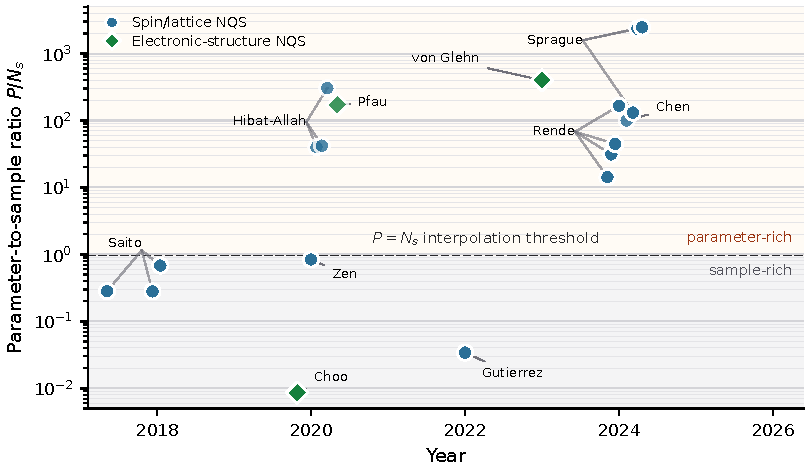
\includegraphics[width=0.95\linewidth]{figures/p_over_ns_literature.pdf}
    \caption{Historical shift in the parameter-to-sample ratio used by VMC/NQS
    calculations. The dashed line marks \(P=N_s\). Marker shape denotes domain:
    circles are spin/lattice NQS and diamonds are electronic-structure NQS.
    Values use each source's parameter-count convention and raw optimizer batch
    size; approximate source-reported counts are included as order-of-magnitude
    points. Sources: \citep{saito2017bosehubbard,
    saitokato2018machine,choo2020fermionic,zen2020critical,hibatallah2020rnn,
    pfau2020ferminet,gutierrez2022real,vonglehn2023psiformer,
    rende2024simple,chen2024empowering,sprague2024variational}.}
    \label{fig:p_over_ns_literature}
\end{figure}

Each SR update solves a linear system with an empirical QGT, which can be
ill-conditioned when estimated from finitely many Monte Carlo
samples. The standard remedy is to add a diagonal shift before solving
\citep{sorella1998green,sorella2001generalized,carleo2017solving}. Historically, this shift was therefore understood mainly as a
numerical conditioning device. In the modern minSR regime, however, the
same operation is applied when the number of variational parameters can far exceed
the number of samples, so its role may be statistical as well as numerical.
This raises the central question of this paper: is the diagonal shift in SR
merely a numerical stabilizer, or is it a statistical filter that makes
overparameterized finite-sample updates generalize, and can this view lead to
better filters than a single $\lambda$?

This question exposes the central tension of modern NQS optimization. More expressive neural quantum states can reduce the \emph{expressivity gap}, the
component of imaginary-time evolution outside the current tangent space.
However, finite-sample SR can also overfit the part of this gap that remains.
The central contributions of this work are:

\begin{itemize}
    \item We formulate SR as a misspecified ridge-regression
    problem. The expressivity gap acts as finite-sample residual noise, yielding
    an exact held-out error identity and a spectral risk approximation for the
    bias--variance role of the diagonal shift \(\lambda\).

    \item We test this mechanism in both exactly tractable small-scale and modern
    large-scale NQS settings. Exact \(4\times4\) matched-noise and matched-state experiments
    separate finite-sample overfitting from expressivity-gap reduction.
    Large-scale shared-checkpoint diagnostics show the predicted U-shaped
    validation risk and monotone variance reduction as \(\lambda\) increases.

    \item We use the filter view to design multi-shift SR (MS-SR), which
    combines independent ridge solves at multiple shifts. Checkpoint-local
    ablations isolate multi-shift filtering, independent-batch averaging, and
    learned stacking. In two equal-budget late-stage branches, fixed-grid MS-SR
    closely tracks SR and finishes below SPRING; robustness and wall-clock
    studies delimit when the additional batches are worthwhile.

\end{itemize}

Section~\ref{sec:ridge} develops the noisy ridge-regression view of SR.
Sections~\ref{sec:small} and~\ref{sec:large_scale} validate its predictions in
exact small-scale and modern large-scale settings. Section~\ref{sec:mssr} shows
that the same perspective leads naturally to MS-SR as a stronger practical
alternative to single-shift SR.

\section{SR as Misspecified Ridge Regression}\label{sec:ridge}

Throughout this section we fix a checkpoint \(\theta\) and assume that the wavefunction and Hamiltonian are real in the
sampling basis for notational simplicity. The complex case is obtained by replacing transposes with
Hermitian conjugates (see Appendix~\ref{app:proofs} for detail).

\paragraph{SR as tangent-space regression.}
Let $\psi_\theta$ be a neural quantum state with Born distribution
\(\pi(x)=|\psi_\theta(x)|^2/\|\psi_\theta\|^2\). Define the centered tangent
features and centered local energy by
\[
    O_c(x)=\nabla_\theta\log\psi_\theta(x)
    -\Expect_\pi[\nabla_\theta\log\psi_\theta],
    \qquad
    H_{\mathrm{loc},c}(x)=H_{\mathrm{loc}}(x)-E(\theta),
\]
where \(H_{\mathrm{loc}}(x)=\langle x|H|\psi_\theta\rangle/
\langle x|\psi_\theta\rangle\) and
\(E(\theta)=\Expect_\pi[H_{\mathrm{loc}}]\). Under normalized imaginary-time
evolution, the log amplitude changes as
\(\Delta\log\psi_\theta(x)=-\eta H_{\mathrm{loc},c}(x)+O(\eta^2)\). A parameter
update \(\theta^+=\theta-\eta\delta\) changes the log amplitude as
\(\log\psi_{\theta^+}(x)-\log\psi_\theta(x)
=-\eta O_c(x)^T\delta+O(\eta^2)\), up to an \(x\)-independent normalization
term. Matching these first-order changes shows that fixed-checkpoint SR fits
tangent predictions \(O_c(x)^T\delta\) to the centered local energy \(H_{\mathrm{loc},c}(x)\).

Writing \(S^\dagger\) for the Moore--Penrose pseudoinverse of
\(S=\Expect_\pi[O_c(x)O_c(x)^T]\), and setting
\(g=\Expect_\pi[O_c(x)H_{\mathrm{loc},c}(x)]\), the ideal fixed-checkpoint SR
direction is the population least-squares solution
\begin{equation}
\label{eq:population_sr_regression}
    \delta^*
    =
    S^\dagger g
    \in
    \argmin_\delta
    \Expect_\pi\!\left[
        \bigl(O_c(x)^T\delta-H_{\mathrm{loc},c}(x)\bigr)^2
    \right].
\end{equation}

\paragraph{Empirical SR as misspecified ridge regression.}
The centered local energy need not be exactly representable by the current
tangent features. We define the tangent-space expressivity gap
$
    \epsilon(x)
    =
    H_{\mathrm{loc},c}(x)-O_c(x)^T\delta^* .
$
The normal equations imply \(\Expect_\pi[\epsilon(x)O_c(x)]=0\), and the gap
variance is
$
    \sigma_{\mathrm{gap}}^2
    =
    \Expect_\pi[\epsilon(x)^2]
    =
    \operatorname{Var}_\pi(H_{\mathrm{loc}})
    -
    g^T S^\dagger g .
$
We call \(\epsilon(x)\) the misspecification noise: it is the part of the
imaginary-time target that lies outside the current tangent space.

Given a Monte Carlo batch \(\mathcal D=\{x_j\}_{j=1}^{N_s}\), empirical SR solves
the ridge problem
\[
    \hat\delta_\lambda=(\hat S+\lambda I)^{-1}\hat g,
    \qquad
    \hat S=\frac1{N_s}\sum_{j=1}^{N_s}O_c(x_j)O_c(x_j)^T,
    \qquad
    \hat g=\frac1{N_s}\sum_{j=1}^{N_s}O_c(x_j)H_{\mathrm{loc},c}(x_j).
\]
Although \(\epsilon(x)\) is orthogonal to the tangent features in population, it
is still present in the sampled targets \(H_{\mathrm{loc},c}(x_j)\). An
overparameterized empirical solve can therefore memorize this residual on the
batch, even though it does not correspond to a generalizable tangent-space
update. In this sense, the expressivity gap behaves as regression noise.

\paragraph{Excess risk analysis.}
Here, we are interested in \(S\)-norm excess risk
$
    \mathcal E_\lambda
    =
    \Expect_{\mathcal D}
    \|\hat\delta_\lambda-\delta^*\|_S^2,
$
where the expectation is over the Monte Carlo batch used to form
\(\hat\delta_\lambda\). This is the out-of-sample error of the checkpoint-local
ridge problem with features \(O_c(x)\), target \(H_{\mathrm{loc},c}(x)\), and
residual noise \(\epsilon(x)\).

The exact bias--variance identity, together with the spectral proxy (see Appendix~\ref{app:proofs} for details), gives
\begin{equation}\label{eq:spectral_risk}
    \mathcal E_\lambda =
    \underbrace{
    \Snorm{\Expect_{\mathcal D}[\hat\delta_\lambda]-\delta^*}
    }_{\text{Bias}}
    +
    \underbrace{
    \Expect_{\mathcal D}
    \Snorm{\hat\delta_\lambda-\Expect_{\mathcal D}[\hat\delta_\lambda]}
    }_{\text{Variance}}
    \approx
    \underbrace{
    \sum_i
    s_i
    \left(\frac{\lambda}{s_i+\lambda}\right)^2
    (\beta_i^*)^2
    }_{\mathcal B_{\mathrm{shrink}}(\lambda)}
    +
    \underbrace{
    \frac{\sigma_{\mathrm{gap}}^2}{N_s}
    \sum_i
    \left(\frac{s_i}{s_i+\lambda}\right)^2
    }_{\mathcal V_{\mathrm{gap}}(\lambda)} ,
\end{equation}
where \(S=V\operatorname{diag}(s_i)V^T\) and
\(\beta_i^*=(V^T\delta^*)_i\). The first term is shrinkage bias: it grows when
\(\lambda\) damps useful components of \(\delta^*\). The second term is
finite-sample variance: it decreases because the same filter suppresses fits to
sampled gap residuals. Thus \(\lambda\) is a statistical regularizer, not only a
numerical tolerance. Standard SR, however, is restricted to the one-parameter
filter family \(s/(s+\lambda)\), motivating the multi-\(\lambda\) filters in
Section~\ref{sec:mssr}.

This \(S\)-norm excess risk is physically relevant because it is closely related to the infidelity, a standard distance measure between quantum states. For bounded updates,
\begin{equation}\label{eq:fs_local_metric}
    \mathcal I_\theta(\delta,\delta')
    =
    1-
    \left|
    \left\langle
        \psi_{\theta-\eta\delta}
        \middle|
        \psi_{\theta-\eta\delta'}
    \right\rangle
    \right|^2
    =
    \eta^2\Snorm{\delta-\delta'}
    +
    O(\eta^3).
\end{equation}
Therefore \(\mathcal E_\lambda\) controls the expected local infidelity between
the ideal population update and the empirical SR update, up to the factor
\(\eta^2\) and higher-order terms.

\paragraph{Large-system diagnostics for excess risk and variance.}
For small systems, the population quantities \(S\), \(\delta^*\),
\(\sigma_{\mathrm{gap}}^2\), and
\(\|\hat\delta_\lambda-\delta^*\|_S^2\) can be computed by exact diagonalization.
This is impossible in the large scale regimes where modern NQS are tuned
and compared. We therefore use two fixed-checkpoint diagnostics that require
only held-out predictions.

The first diagnostic is a validation residual. Let
\(\mathcal D_{\mathrm{val}}\) be independent of the batches used to compute the
SR updates. Since
\(H_{\mathrm{loc},c}(x)=O_c(x)^T\delta^*+\epsilon(x)\) with
\(\Expect_\pi[\epsilon(x)O_c(x)]=0\), any fixed update \(\delta\) satisfies
\begin{equation}\label{eq:rval_decomp}
    R_{\mathrm{val}}(\delta)
    =
    \frac1{|\mathcal D_{\mathrm{val}}|}
    \sum_{x\in\mathcal D_{\mathrm{val}}}
    \bigl(O_c(x)^T\delta-H_{\mathrm{loc},c}(x)\bigr)^2,
    \qquad
    \Expect_{\mathcal D_{\mathrm{val}}}
    \left[R_{\mathrm{val}}(\delta)\right]
    =
    \|\delta-\delta^*\|_S^2+\sigma_{\mathrm{gap}}^2 .
\end{equation}
Thus, for independent SR updates
\(\hat\delta_{\lambda,1},\dots,\hat\delta_{\lambda,m}\) at the same checkpoint,
we use
\(\widehat{\mathcal E}_{\mathrm{val}}(\lambda)
=m^{-1}\sum_{j=1}^m R_{\mathrm{val}}(\hat\delta_{\lambda,j})\). Its expectation
is \(\mathcal E_\lambda+\sigma_{\mathrm{gap}}^2\), so it tracks excess risk plus the expressivity-gap.

The second diagnostic measures how much the update varies across independent
training batches. With
\(\bar\delta_\lambda=m^{-1}\sum_j\hat\delta_{\lambda,j}\), define
\begin{equation}\label{eq:vmb_def}
    \mathcal V_{\mathrm{mb}}(\lambda)
    =
    \frac1{m-1}
    \sum_{j=1}^m
    \frac1{|\mathcal D_{\mathrm{val}}|}
    \sum_{x\in \mathcal D_{\mathrm{val}}}
    \bigl(O_c(x)^T(\hat\delta_{\lambda,j}-\bar\delta_\lambda)\bigr)^2 .
\end{equation}
As \(m\) and the validation batch grow, this converges to the variance component
of the excess risk. Both diagnostics are practical at large scale because they only require
held-out tangent-feature predictions. Since they do not require forming or
solving a validation QGT or NTK system, they can be evaluated on validation
batches much larger than the SR training batch with modest computational cost.

Together, these diagnostics test the bias and variance role of the diagonal
shift at a fixed checkpoint. Increasing \(\lambda\) first suppresses noisy
small-eigenvalue directions, so \(\widehat{\mathcal E}_{\mathrm{val}}\) can
decrease as variance falls. Once \(\lambda\) also suppresses useful update
directions, shrinkage bias dominates and the validation curve rises. The
predicted signature is therefore a U-shaped
\(\widehat{\mathcal E}_{\mathrm{val}}\) with a monotonically decreasing
\(\mathcal V_{\mathrm{mb}}\).

\section{Small-scale Dissection of Expressivity and Overfitting in SR}\label{sec:small}

\begin{figure}[t]
    \centering
    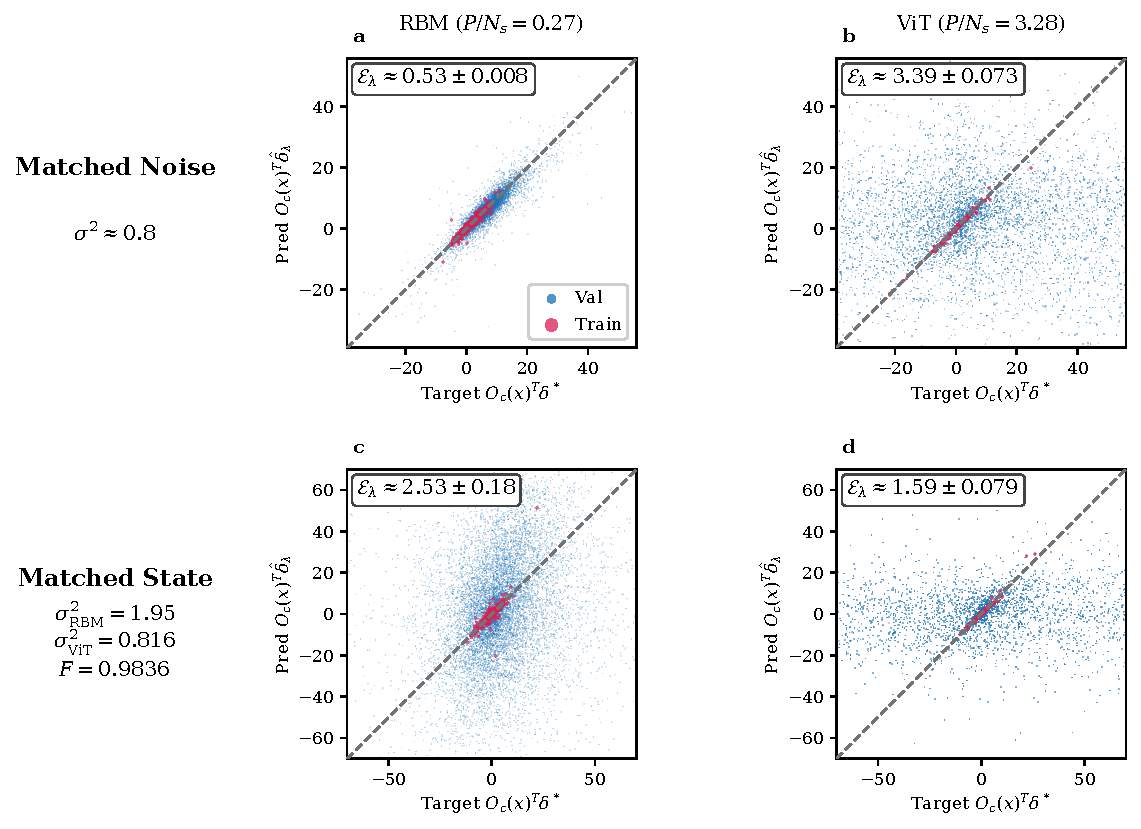
\includegraphics[width=0.95\textwidth]{figures/figure2.pdf}
    \caption{Small-scale SR risk geometry for the periodic \(4\times4\)
    \(J_1\)-\(J_2\) model at \(N_s=4096\) and \(\lambda=10^{-9}\). Panels compare
    empirical predictions (y-axis) with ideal tangent-space
    predictions (x-axis). Matched-noise exposes ViT overfitting at
    comparable noise \(\sigma_{\mathrm{gap}}^2\). Matched-state shows the ViT's larger tangent space reduces
    the expressivity gap and excess risk. Reported uncertainties are one sample
    standard error across the $100$ matched-noise or $10$ matched-state
    independently resampled training batches.}
    \label{fig:smallscale_paradox}
\end{figure}

This section tests the mechanism of Section~\ref{sec:ridge} in an exactly
diagonalizable spin-$1/2$ system. We use the periodic $4\times4$ square-lattice
$J_1$-$J_2$ Heisenberg model
$
    H
    =
    J_1\sum_{\langle i,j\rangle}\mathbf S_i\cdot\mathbf S_j
    +
    J_2\sum_{\langle\!\langle i,j\rangle\!\rangle}
    \mathbf S_i\cdot\mathbf S_j .
$
We set $J_2/J_1=0.5$, which is a strongly frustrated point. Here $\mathbf S_i$ is the spin-$1/2$ operator at site $i$, while
$\langle i,j\rangle$ and $\langle\!\langle i,j\rangle\!\rangle$ denote
nearest-neighbor and next-nearest-neighbor bonds.

All SR solves use a fixed sample budget of $N_s=4096$. We compare an
underparameterized RBM with $P/N_s=0.27$ to an overparameterized Vision
Transformer with $P/N_s=3.28$. For the selected comparisons, we draw $100$
independent training batches for matched noise and $10$ for matched state,
then compute the corresponding empirical shifted-SR updates
$\hat\delta_\lambda(\mathcal D_b)$. Because the $4\times4$ system is exactly
diagonalizable, the population QGT $S$, the population target update
$\delta^*$, and the expressivity-gap variance $\sigma_{\mathrm{gap}}^2$ are
computed exactly over the full Hilbert space. We estimate the excess risk by
averaging $\|\hat\delta_\lambda(\mathcal D_b)-\delta^*\|_S^2$ over the
independent batches, and report the sample mean with one sample standard error
(the trial sample standard deviation divided by the square root of the number
of batches). Thus, unlike the
large-system diagnostic $\widehat{\mathcal E}_{\mathrm{val}}$, this small-scale
measurement uses the exact population geometry rather than a validation
approximation. We use the near-ridgeless shift
$\lambda=10^{-9}$, which deliberately exposes the tendency of empirical SR to
fit sample-specific expressivity-gap noise.
Equivalently, Figure~\ref{fig:smallscale_paradox} visualizes this excess risk
pointwise: deviations from the diagonal measure how much the empirical
prediction $O_c(x)^T\hat\delta_\lambda$ differs from the ideal tangent-space
prediction $O_c(x)^T\delta^*$ on training (red) and held-out (blue) configurations.

The experiment separates two effects that are coupled.
The matched-noise comparison keeps $\sigma_{\mathrm{gap}}^2$ approximately fixed
and tests the finite-sample cost of a larger tangent space. The matched-state
comparison keeps the represented wavefunction approximately fixed and tests the
expressivity benefit of the larger tangent space. Full model and optimization
details are given in Appendix~\ref{app:small}.

\paragraph{Matched-noise comparison.}
To test the finite-sample cost of overparameterization, we select independently
trained RBM and ViT checkpoints with comparable expressivity-gap variance. In
Figure~\ref{fig:smallscale_paradox} panel (a) and (b), both values of
$\sigma_{\mathrm{gap}}^2$ are close to $0.8$. At
$\lambda=10^{-9}$, the RBM remains close to the ideal population update, with
$\mathcal E_\lambda\approx0.53\pm0.008$. The ViT has comparable
misspecification noise, but its empirical solve fits the sampled residual much
more strongly, increasing the excess-risk estimate to
$\mathcal E_\lambda\approx3.39\pm0.073$. This is the variance-driven failure mode
predicted by Eq.~\eqref{eq:spectral_risk}. When the expressivity gap is held fixed,
a larger tangent space gives the empirical SR update more directions in which to
fit sample-specific noise.

\paragraph{Matched-state comparison.}
To isolate the benefit of a larger tangent space, we freeze a partially
converged RBM checkpoint and fit a ViT to represent the same quantum state by
minimizing infidelity~\cite{sinibaldi2023unbiasing,gravina2410neural}. The two represented states have fidelity \(F\geq0.98\).
Thus the wavefunction is nearly fixed, while the tangent space changes. Under
this matched-state protocol, ViT's larger tangent space lowers the
expressivity gap variance from \(\sigma_{\mathrm{gap}}^2=1.95\) to \(0.816\).
The excess-risk estimate also decreases from
\(\mathcal E_\lambda\approx2.53\pm0.18\) to
\(\mathcal E_\lambda\approx1.59\pm0.079\). Thus overparameterization can improve
SR generalization when its additional tangent directions reduce enough
misspecification noise.

Together, these comparisons show the central tension of overparameterized SR.
A larger model improves the update by reducing the expressivity gap, but it also worsens the update when a comparable gap remains and the finite-sample
solve overfits it. This emphasizes the role of the diagonal shift $\lambda$ as a statistical filter that controls how much sampled
gap noise enters the SR update. 

\section{Large-Scale Checkpoint Diagnostics of the Noisy-Ridge Mechanism}
\label{sec:large_scale}

\begin{figure}[t]
    \centering
    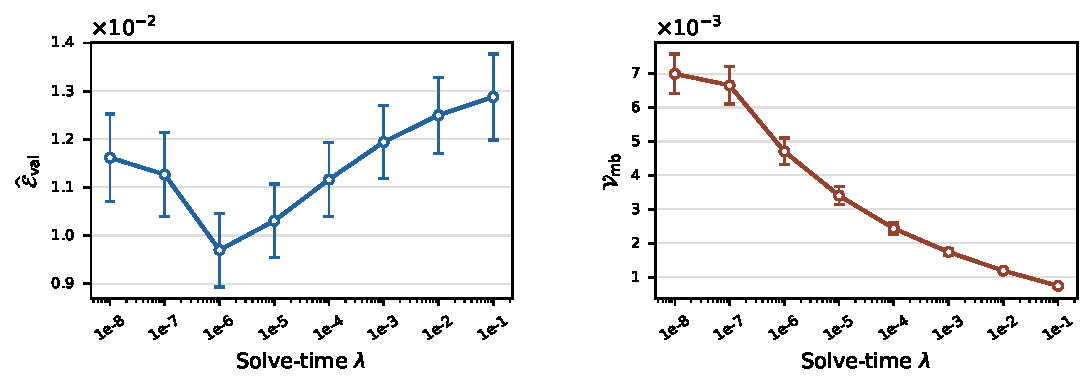
\includegraphics[width=0.95\textwidth]{figures/figure3_tfim_fixed_data.pdf}
    \caption{Large-scale shared-checkpoint test of the noisy-ridge mechanism on
    the periodic \(L=100\) transverse-field Ising model with \(h\) ranging from \(0.8\) to \(1.2\) with foundational NQS.
    A fixed set of late-training checkpoints is reused while only the
    solve-time shift $\lambda$ is varied. $\widehat{\mathcal E}_{\mathrm{val}}$ is U-shaped, while $\mathcal V_{\mathrm{mb}}$ decreases monotonically with
    $\lambda$, matching the two predictions of Section~\ref{sec:ridge}. Error
    bars are one standard error across the ten checkpoint-level means.}
    \label{fig:large_scale_ucurve}
\end{figure}

The exact $4\times4$ study isolates the noisy-ridge mechanism using population
quantities. We next test whether the same mechanism remains visible in modern
overparameterized NQS, where the population QGT, population SR direction, and
expressivity-gap variance are unavailable. We therefore test the mechanism using the
checkpoint-local diagnostics introduced in Section~\ref{sec:ridge}.

We use a foundation neural quantum state (FNQS) on the $L=100$ periodic
one-dimensional transverse-field Ising model (TFIM) family,
$
    H=-h\sum_i X_i-\sum_i Z_iZ_{i+1},
$
with $h\in[0.8,1.2]$. A single conditional
wave function $\log\psi_\theta(x;h)$ is trained across many Hamiltonian
parameters, so the SR update must aggregate information over a family of
Hamiltonians. The model has
$P=198{,}144$ parameters, while each SR step uses a batch of
$N_s=12{,}000$ samples, split over $6000$ training $h$ values with two spin
configurations per field. We use the same architectural and sampler setting as
\citet{rende2025foundation} (see Appendix~\ref{app:large} for experimental details).

The diagnostic experiment uses a shared-checkpoint protocol. We first take ten
late-training checkpoints from the run trained with
$\lambda_{\mathrm{train}}=10^{-4}$. These checkpoints are then held fixed. At
each checkpoint, we perform an offline sweep over the solve-time shift
$
    \lambda\in\{10^{-8},10^{-7},\ldots,10^{-1}\},
$
recomputing standard SR updates on fresh resampled batches for each value of
$\lambda$. This design keeps the wave function, tangent geometry, and
expressivity-gap fixed while varying only the ridge penalty. It therefore
tests the local bias--variance mechanism directly, not the different training trajectories.

For each checkpoint and each diagnostic shift, we construct $m=20$ independent
standard-SR updates from independently resampled training batches. The validation
diagnostic uses $120{,}000$ held-out samples, consisting of $6000$ held-out
$h$ values, disjoint from the training $h$ values, and $20$ spin configurations per
$h$ value. Predictions are centered separately for each $h$ value, since each
Hamiltonian parameter has its own local-energy distribution. The validation pass
then estimates both $\widehat{\mathcal E}_{\mathrm{val}}$ and
$\mathcal V_{\mathrm{mb}}$ without forming or solving any validation QGT system.

Figure~\ref{fig:large_scale_ucurve} shows the fixed-checkpoint signature
predicted by the noisy-ridge view. The
$\hat{\mathcal{E}}_{\mathrm{val}}$ curve is U-shaped in \(\lambda\), while
\(\mathcal V_{\mathrm{mb}}\) decreases as \(\lambda\) increases. Since all
shifts are evaluated on the same checkpoints, this trend reflects the
solve-time ridge filter rather than different training trajectories. Small
shifts leave useful directions nearly undamped but fit more batch-dependent
noise. Large shifts reduce this variance but also shrink useful population
directions.

\section{Multi-Shift SR for Statistical Filtering and Variance Reduction}
\label{sec:mssr}

Motivated by the noisy-ridge view, we introduce multi-shift SR (MS-SR), an
optimizer that replaces the single shifted SR solve with a mixture of shifted
SRs computed on independent batches. Standard SR uses one ridge scale
and therefore applies the same spectral filter \(s/(s+\lambda)\) to every QGT
eigendirection. MS-SR instead combines several regularization scales, while the
independent batches decorrelate finite-sample errors.

At checkpoint \(\theta_t\), MS-SR draws \(K\) independent batches
\(\mathcal D_1,\ldots,\mathcal D_K\), chooses shifts \(\lambda_k\) from
empirical NTK-spectrum quantiles, and computes candidate updates
\(\hat\delta_k=\minSR(\mathcal D_k,\lambda_k)\). It then forms
\(\hat\delta_{\mathrm{MS}}=\sum_{k=1}^K w_k\hat\delta_k\), with
\(\mathbf w\in\Delta^{K-1}\). The weights are selected by leave-one-batch-out
stacking, so each candidate update is evaluated only on batches that were not
used to compute it. The full procedure is given in
Algorithm~\ref{alg:mssr_appendix} in Appendix~\ref{app:mssr}.

This construction has a simple bias--variance interpretation. For fixed shifts
and mixture weights, define
$
    \bar\delta_k
    =
    \Expect_{\mathcal D_k}
    \left[
        \hat\delta_k
    \right].
$
Then the excess risk decomposes exactly as
\begin{equation}
\label{eq:mssr_decomp}
    \Expect
    \left[
        \left\|
            \hat\delta_{\mathrm{MS}}-\delta^*
        \right\|_S^2
    \right] =
    \left\|
        \sum_{k=1}^K
        w_k\bar\delta_k
        -
        \delta^*
    \right\|_S^2 +
    \Expect
    \left[
        \left\|
            \sum_{k=1}^K
            w_k
            \left(
                \hat\delta_k
                -
                \bar\delta_k
            \right)
        \right\|_S^2
    \right].
\end{equation}
The first term is the bias of the average filter. The second term is the
finite-batch variance of the average update. MS-SR targets both terms: multiple
shifts enlarge the filter class, while independent batches reduce the variance
of the noisy solves.

\paragraph{Why multiple shifts help.}
\label{par:multi_lambda}

Consider the population spectral approximation from
Section~\ref{sec:ridge}. If
\(S=V\operatorname{diag}(s_i)V^T\), then a single ridge solve applies the
filter
$
    f_{\lambda}(s)
    =
    {s}/{(s+\lambda)}
$
to each eigendirection. A convex mixture of ridge solves applies instead
$
    f_{\mathbf w,\boldsymbol\lambda}(s)
    =
    \sum_k
    w_k
    {s}/{(s+\lambda_k)}.
$
Thus MS-SR is still a spectral filter, but it is no longer restricted to the
single-shift family.

The difference is clearest at the two ends of the spectrum. For small \(s\),
\(f_{\mathbf w,\boldsymbol\lambda}(s)
=s\sum_k w_k/\lambda_k+O(s^2)\). For large \(s\),
\(f_{\mathbf w,\boldsymbol\lambda}(s)
=1-(\sum_k w_k\lambda_k)/s+O(s^{-2})\).
With a single shift, the same \(\lambda\) controls both the suppression of
low-eigenvalue directions and the residual shrinkage of high-eigenvalue
directions. On the other hand, these two behaviors can be tuned separately with multiple shifts. 
This can improve the aggregate bias--variance tradeoff when useful update directions
and noise-sensitive directions are not controlled well by the same shift.
\begin{figure}[t]
    \centering
    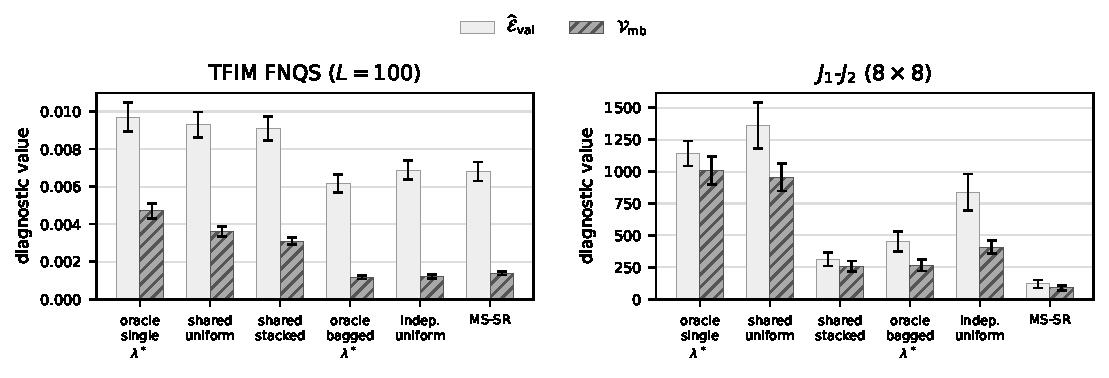
\includegraphics[width=\textwidth]{figures/figure4_mssr_ablation_oracle.pdf}
    \caption{Checkpoint-local ablations for the ingredients of MS-SR at $K=4$.
    Paired bars show raw $\widehat{\mathcal{E}}_\mathrm{val}$ and $\mathcal{V}_{\mathrm{mb}}$
    averaged over ten fixed source checkpoints; error bars are one standard
    error across checkpoints. Both single SR and bagged SR are
    \emph{evaluation-oracle} baselines using the validation-optimal
    $\lambda^*$ at each checkpoint. MS-SR selects its NTK-quantile shift grid
    without validation tuning.}
    \label{fig:mssr_diagnostics}
\end{figure}
\paragraph{Why independent batches help.}
\label{par:multi_batch}

The second term in Eq.~\eqref{eq:mssr_decomp} depends on the correlations
between candidate updates. If the candidates are computed on independent
batches, the cross terms vanish and
$
    \Expect
        \|
            \sum_k
            w_k
            (
                \hat\delta_{\lambda_k}^{(k)}
                -
                \bar\delta_{\lambda_k}
            )
        \|_S^2
    =
    \sum_k
    w_k^2
    \hspace{0.1em}
    \Expect
        \|
            \hat\delta_{\lambda_k}^{(k)}
            -
            \bar\delta_{\lambda_k}
        \|_S^2.
$
For uniform weights, this is a factor-\(K\) reduction of the average
single-batch variance in the ideal independent-batch limit.

Independent batches produce a bagging-like effect by decorrelating the sampling
noise across candidate updates. If all \(K\) shifts are solved on the same
batch, the resulting candidates can still enrich the spectral filter, but their
sampling errors remain shared. Consequently, the variance-reduction effect is lost.
A single larger batch of size \(KN_s\) would also reduce variance, but it is substantially more expensive
computationally, with cost \(O(K^3N_s^3)\). On the other hand,
\(K\) independent solves at batch size \(N_s\) cost only \(O(KN_s^3)\) and can
be run in parallel. MS-SR obtains the statistical benefit of a larger batch without paying the
cubic cost of a single enlarged solve.


\paragraph{Shift and weight selection.}
\label{par:mssr_weights}

MS-SR first chooses the shifts and then fits the mixture weights. In our
checkpoint-local \(K=4\) experiments, the shifts are the empirical NTK-spectrum
quantiles \(\{0.9,0.7,0.4,0.1\}\). These quantiles place the ridge transition
scale at several parts of the
empirical spectrum, producing candidate updates with different bias--variance
tradeoffs rather than relying on a single regularization. The online comparison
instead uses the predeclared fixed grid
\(\{10^{-2},10^{-3},10^{-4},10^{-5}\}\).

Given these shifts, Algorithm~\ref{alg:mssr_appendix} uses leave-one-batch-out stacking
to choose the weights. Each candidate update is evaluated on batches that were
not used to compute it. The weights minimize the held-out residual between
tangent-feature predictions and centered local energies, giving a direct
estimate of the regression risk from Eq.~\eqref{eq:rval_decomp}.


\paragraph{Ablation study of MS-SR.}
\label{par:mssr_ablations}

Figure~\ref{fig:mssr_diagnostics} compares six checkpoint-local updates using
ten fixed checkpoints from TFIM and from the $8\times8$ square-lattice
$J_1$-$J_2$ model at $J_2/J_1=0.5$. The single and bagged baselines both use
the per-checkpoint validation minimizer $\lambda^*$ over
$\{10^{-8},\ldots,10^{-1}\}$; bagging averages four independent solves at that
same $\lambda^*$. These are deliberately strong diagnostic oracles, not online
methods. The shared-batch variants isolate multi-shift filtering, the
independent-batch variants isolate averaging, and MS-SR adds stacking.

The ordering is regime-dependent. On TFIM, where $\lambda^*=10^{-6}$ at all
ten checkpoints, oracle bagging has lower validation risk than MS-SR
($0.00617$ versus $0.00680$). At the training shift $10^{-4}$, however, bagging
has risk $0.00933$, and MS-SR is lower on all ten checkpoints. On the harder
$J_1$-$J_2$ checkpoints, MS-SR has risk $120.1$, versus $451.0$ for oracle
bagging, a $73\%$ reduction. Thus the additional shifts are most useful when
no stable single shift suffices; when the validation-optimal shift is stable,
single-shift bagging can be preferable. Appendix~\ref{app:mssr_robustness}
reports the fixed-shift, $K$, quantile, and source-shift studies, and
Appendix~\ref{app:mssr_cost} reports measured wall time.

\paragraph{Equal-budget online comparison.}
\label{par:mssr_online}
\begin{figure}[t]
    \centering
    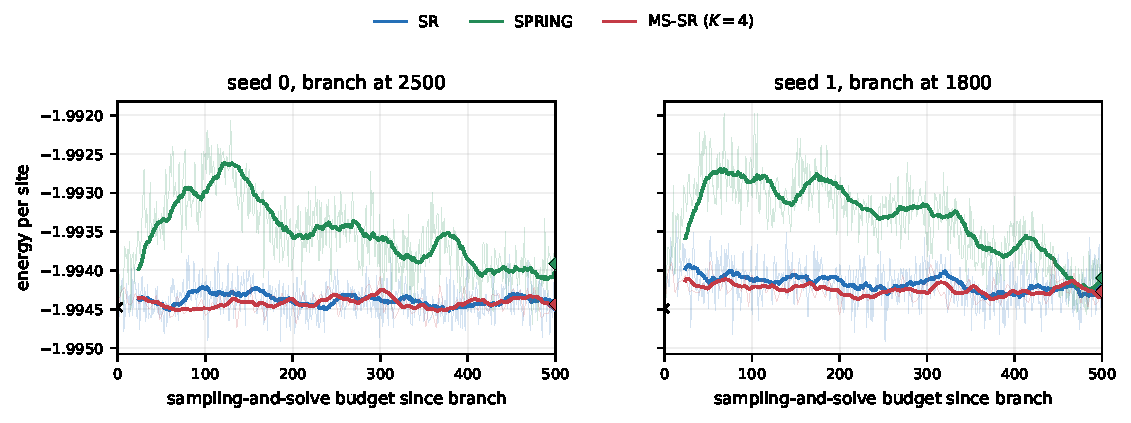
\includegraphics[width=\textwidth]{figures/figure5_equal_budget_online.pdf}
    \caption{Equal-budget late-stage online comparison on the $8\times8$
    $J_1$-$J_2$ model with a no-symmetry ViT. Each panel branches SR, SPRING,
    and fixed-grid MS-SR from identical parameters. One SR or SPRING update is
    one budget unit; one $K=4$ MS-SR update is four. Faint lines are raw
    training-energy estimates and solid lines are rolling means over a common
    25-budget-unit window. Diamonds are audited fresh-chain
    endpoint evaluations; bars are one conservative reported Monte Carlo
    standard error, not variation across seeds.}
    \label{fig:mssr_equal_budget_online}
\end{figure}

Figure~\ref{fig:mssr_equal_budget_online} compares two controlled late-stage
branches at equal sampling-and-solve budget. Each arm receives $500$ units, so
SR and SPRING take $500$ updates while MS-SR takes $125$.
For seed 0 (branch step 2500), MS-SR $-1.9944365\mathbin{\pm}7.06\times10^{-6}$, SR $-1.9944498\mathbin{\pm}6.86\times10^{-6}$, SPRING $-1.9939130\mathbin{\pm}8.36\times10^{-6}$. The numerical endpoint ordering (lower is better) is SR $<$ MS-SR $<$ SPRING; MS-SR minus SR is $+0.0000133$ per site ($+1.36$ combined endpoint Monte Carlo standard errors); MS-SR minus SPRING is $-0.0005235$ per site ($-47.84$ combined endpoint Monte Carlo standard errors).
For seed 1 (branch step 1800), MS-SR $-1.9942723\mathbin{\pm}7.83\times10^{-6}$, SR $-1.9942534\mathbin{\pm}7.88\times10^{-6}$, SPRING $-1.9940982\mathbin{\pm}8.02\times10^{-6}$. The numerical endpoint ordering (lower is better) is MS-SR $<$ SR $<$ SPRING; MS-SR minus SR is $-0.0000189$ per site ($-1.70$ combined endpoint Monte Carlo standard errors); MS-SR minus SPRING is $-0.0001741$ per site ($-15.53$ combined endpoint Monte Carlo standard errors).
These are two individual branched trajectories; the endpoint uncertainties
measure Monte Carlo evaluation error and do not estimate across-seed variation.


\section{Related Work}

Neural quantum states have evolved rapidly from compact RBM-like ans\"atze to
deep convolutional, recurrent, transformer-based, fermionic, and
foundation-style wave functions
\citep{carleo2017solving, hibatallah2020rnn, pfau2020ferminet,
vonglehn2023psiformer, nomura2021dirac, rende2024simple,
nutakki2025design, rende2025foundation}. Autoregressive NQS provide a
complementary route to scalability because their normalized factorization
permits sampling from the model Born distribution rather than
Markov-chain sampling \citep{hibatallah2020rnn}. This changes the sampling and
autocorrelation structure of VMC, but it does not remove the finite-sample
nature of SR, since QGTs and forces are still estimated from finite samples.

SR is the natural-gradient method of VMC, with the QGT playing the role of the
Fisher metric on the variational manifold
\citep{sorella1998green, sorella2001generalized, carleo2017solving}. Recent sample-space formulations, including minSR, avoid forming the full
\(P\times P\) QGT and instead solve an \(N_s\times N_s\) kernel system, making
SR practical for highly overparameterized NQS
\citep{chen2024empowering, rende2024simple}. SPRING builds on this view with a
Kaczmarz-inspired projected-increment update that reuses information across
minibatches to accelerate convergence \citep{goldshlager2024spring,goldshlager2025sketch}. These
methods improve the cost and convergence of SR, while our focus is the
statistical filtering role of the diagonal shift.

A parallel line of work approximates the QGT or Fisher metric structurally.
KFAC uses Kronecker-factored curvature approximations and has been important in
FermiNet-style electronic-structure VMC
\citep{martens2015optimizing, pfau2020ferminet}. Block-diagonal
QGT methods partition the NQS metric by network layers, preserving intra-layer
curvature while suppressing noisy cross-layer correlations
\citep{shokry2025blockqgt}. These approaches change the metric approximation.
MS-SR is complementary: it keeps the sample-space SR geometry but replaces
the single-shift ridge filter with a data-adaptive mixture of shifted solves.

Our analysis connects SR to random-design ridge regression
\citep{hsu2012random}. In this view, the local-energy target is generally
misspecified by the current tangent space, and the expressivity gap
acts as the irreducible residual noise. Sketch-and-project and Kaczmarz
interpretations clarify the structure of the overparameterized linear solve
\citep{strohmer2009randomized, goldshlager2024spring, goldshlager2025sketch}. The
present work identifies the statistical source of the noise being fitted and
uses that view to design richer spectral filters for SR.

\section{Conclusion}

Modern NQS optimization has entered a finite-sample, parameter-rich regime. In
this regime the diagonal shift in SR is not just a safeguard against an
ill-conditioned empirical QGT. It is also the spectral regularizer that
determines how much of the sampled tangent-space target is trusted. By recasting
a single SR step as misspecified ridge regression, we identified the
tangent-space expressivity gap as the effective noise source: it is orthogonal
to the tangent features in population, but it is present in every finite batch
and can be fitted by overparameterized empirical solves.

This viewpoint explains the apparent tension observed throughout the paper.
Larger models improve SR when their tangent spaces reduce the expressivity gap,
but they can also amplify finite-sample overfitting when a comparable gap
remains. The exact small-system experiments and the large
fixed-checkpoint diagnostics show the same bias--variance structure across
scales.

The filter perspective also leads to MS-SR, which mixes independent ridge
solves at multiple shifts. Independent batches reduce variance, multiple shifts
enlarge the filter class, and stacking adapts the mixture to the local
checkpoint. The equal-budget online branches test whether this local advantage
translates to training outcomes late in optimization. Across the two tested
branches, MS-SR closely tracks SR, with opposite numerical ordering, and ends
below SPRING in both; these are trajectory-level outcomes rather than a
population optimizer ranking. The checkpoint ablations identify counter-regimes
in which an oracle single shift is better.
For the eigensolver implementation studied here, $K=4$ bagged SR and MS-SR take
$4.00\times$ and $4.04\times$ the wall time of single SR, respectively; the
method-specific overhead beyond the common four batches and solves is about
$1\%$.

\paragraph{Limitations.}\label{sec:limitations}
The theory is checkpoint-local and its factor-$K$ variance statement requires
independent candidate batches; autocorrelation reduces the effective sample
size, and shared chains can correlate candidates. The online study covers two
late branches of one $8\times8$ system rather than a broad optimizer benchmark,
and MS-SR is not uniformly superior: oracle bagging wins on TFIM, and the
Shastry--Sutherland negative result in Appendix~\ref{app:ssm_negative} shows
failure when the shift grid is misspecified. MS-SR also spends $K$ times the
sampling and solve budget of single SR. The timing ratios come from one H100
hardware/software stack and need not transfer unchanged. The evaluation-oracle
baselines intentionally select $\lambda^*$ on the same validation stream used
to report risk, so they contain selection leakage. Endpoint error bars are
finite-round MCMC standard errors and do not represent between-branch
variation. These results therefore support a
diagnostic, regime-dependent filtering rule rather than a universal optimizer
ranking.

Overall, overparameterization should not be avoided in NQS, but
it should be treated with the right statistical regularization. Treating SR as a
statistical filtering problem provides both a diagnostic language for
understanding existing optimizers and a design principle for building more
reliable ones.

\clearpage
\phantomsection\label{main:references:start}
\bibliographystyle{plainnat}
\bibliography{references}

\clearpage
\appendix
\phantomsection\label{app:start}
\section{Code and Data Availability}\label{app:code}
The public repository containing the code, compact artifacts, and figure
regeneration tools for this work is
\url{https://github.com/takh04/sr_filter}.
The experimental tools were developed on top of NetKet, an open-source
neural-quantum-state and variational Monte Carlo library distributed under the
Apache License 2.0 \citep{vicentini2022netket}.

\section{Fixed-Checkpoint SR Regression Identities}\label{app:proofs}

This appendix gives the derivations behind Section~\ref{sec:ridge}. All
statements are checkpoint-local: the wavefunction \(\psi_\theta\), sampling
distribution \(\pi\), QGT, and tangent features are held fixed while only the
Monte Carlo batch used to estimate the SR direction varies. We write
\(\Snorm{u}=u^T S u\). Since \(S\) may be singular, null QGT directions do not
change tangent predictions and have zero \(S\)-seminorm. Throughout,
\(^{\dagger}\) denotes the Moore--Penrose pseudoinverse; Hermitian adjoints are
written explicitly as \(\overline{u}^{\,T}\).

\subsection{Real and complex conventions}

The main text assumes real wavefunctions and real tangent features in the
sampling basis. Then
\[
    S=\Expect_\pi[O_c(x)O_c(x)^T],
    \qquad
    g=\Expect_\pi[O_c(x)H_{\mathrm{loc},c}(x)] .
\]
The fixed-checkpoint population problem is the ordinary least-squares problem
\[
    \min_\delta
    \Expect_\pi\!\left[
        \left(O_c(x)^T\delta-H_{\mathrm{loc},c}(x)\right)^2
    \right],
\]
and its minimum-norm solution is \(\delta^*=S^\dagger g\).

For complex wavefunctions, let
\[
    O_c(x)=\nabla_\theta\log\psi_\theta(x)
    -\Expect_\pi[\nabla_\theta\log\psi_\theta],
    \qquad
    H_{\mathrm{loc},c}(x)=H_{\mathrm{loc}}(x)-\Expect_\pi H_{\mathrm{loc}} .
\]
The Hermitian QGT and force are
\[
    Q=\Expect_\pi[\overline{O_c(x)}\,O_c(x)^T],
    \qquad
    f=\Expect_\pi[\overline{O_c(x)}\,H_{\mathrm{loc},c}(x)] .
\]
For complex parameter increments \(\delta\in\mathbb C^p\), the regression loss is
\(\Expect_\pi|O_c(x)^T\delta-H_{\mathrm{loc},c}(x)|^2\), the normal equations are
\(Q\delta=f\), and the corresponding seminorm is
\(\overline{\delta}^{\,T}Q\delta=\Expect_\pi|O_c(x)^T\delta|^2\). For real parameter
increments in a complex wavefunction, minimizing the same modulus-squared loss
over \(\delta\in\mathbb R^p\) gives $\operatorname{Re}[Q\,\delta]=\operatorname{Re}[f].$
Equivalently, one stacks the real and imaginary residuals and solves an ordinary
real least-squares problem. Thus the real-parameter SR equation uses
\(S=\operatorname{Re}[Q]\) and \(g=\operatorname{Re}[f]\). The derivations below are
written in the real convention. In the complex convention, replace scalar
squares by modulus squares and replace the \(S\)-seminorm by the corresponding
real or Hermitian QGT seminorm.

\subsection{Validation and variance identities}

Let \(\delta^*\) be the population least-squares SR direction and define
\[
    \epsilon(x)=H_{\mathrm{loc},c}(x)-O_c(x)^T\delta^* .
\]
The population normal equations give
\(\Expect_\pi[O_c(x)\epsilon(x)]=0\). Hence, for any fixed direction
\(\delta\),
\[
\begin{aligned}
    \Expect_\pi\!\left[
        \left(O_c(x)^T\delta-H_{\mathrm{loc},c}(x)\right)^2
    \right]
    &=
    \Expect_\pi\!\left[
        \left(O_c(x)^T(\delta-\delta^*)-\epsilon(x)\right)^2
    \right] \\
    &=
    \Snorm{\delta-\delta^*}
    +\sigma_{\mathrm{gap}}^2,
\end{aligned}
\]
where \(\sigma_{\mathrm{gap}}^2=\Expect_\pi[\epsilon(x)^2]\). Thus an
independent held-out residual estimates the \(S\)-excess risk up to the constant
expressivity-gap term.

For a random diagnostic update \(Z=\hat\delta_\lambda\) computed by resampling
an SR batch at the same checkpoint, let \(\mu=\Expect_{\mathcal D}Z\). Adding and
subtracting \(\mu\) gives
\[
\begin{aligned}
    \mathcal E_\lambda
    =
    \Expect_{\mathcal D}\Snorm{Z-\delta^*}
    &=
    \Snorm{\mu-\delta^*}
    +
    \Expect_{\mathcal D}\Snorm{Z-\mu} .
\end{aligned}
\]
The cross term vanishes because \(\Expect_{\mathcal D}[Z-\mu]=0\). This is the
usual squared-bias plus variance decomposition, with distances measured in the
checkpoint QGT seminorm.

Finally, let \(Z_1,\ldots,Z_m\) be independent copies of \(Z\) and
\(\bar Z=m^{-1}\sum_j Z_j\). The standard sample-variance identity holds in the
same seminorm:
\[
    \Expect\left[
        \frac1{m-1}\sum_{j=1}^m\Snorm{Z_j-\bar Z}
    \right]
    =
    \Expect\Snorm{Z-\mu} .
\]
Equivalently,
\[
    \frac1{m-1}\sum_{j=1}^m\Snorm{Z_j-\bar Z}
    =
    \frac1{\binom m2}
    \sum_{a<b}\frac12\Snorm{Z_a-Z_b} .
\]
Replacing each \(S\)-seminorm prediction norm by its empirical held-out average
\( |\mathcal D_{\mathrm{val}}|^{-1}\sum_x (O_c(x)^T\cdot)^2\) gives the
multi-batch diagnostic used in the main text.

\subsection{Spectral filter proxy}

On the non-null QGT subspace, write
\(S=V\operatorname{diag}(s_i)V^T\) with \(s_i>0\), and let
\(\beta_i^*=(V^T\delta^*)_i\). The population ridge direction is
\[
    \delta_\lambda=(S+\lambda I)^{-1}g
    =(S+\lambda I)^{-1}S\delta^* .
\]
Therefore
\[
    \delta_\lambda-\delta^*
    =
    -\lambda(S+\lambda I)^{-1}\delta^* ,
\]
and the exact population shrinkage bias is
\[
    \Snorm{\delta_\lambda-\delta^*}
    =
    \sum_i
    s_i
    \left(\frac{\lambda}{s_i+\lambda}\right)^2
    (\beta_i^*)^2 .
\]

The scalar variance term in \eqref{eq:spectral_risk} is a reference calculation,
not an assumption needed by the diagnostics. To isolate the residual-noise
contribution, write
\[
    \hat g=\hat S\delta^*+\hat\xi,
    \qquad
    \hat\xi
    =
    \frac1{N_s}\sum_{j=1}^{N_s}O_c(x_j)\epsilon(x_j),
    \qquad
    \Expect[\hat\xi]=0 .
\]
If one ignores the covariance-estimation fluctuation in \(\hat S\) and replaces
the empirical inverse by \(A_\lambda=(S+\lambda I)^{-1}\), then
\[
    \hat\delta_\lambda-\delta_\lambda
    \approx
    A_\lambda\hat\xi .
\]
Let
\(\Sigma_\epsilon=\Expect_\pi[O_c(x)O_c(x)^T\epsilon(x)^2]\). The force-noise
proxy is then
\[
    \Expect_{\mathcal D}
    \Snorm{\hat\delta_\lambda-\delta_\lambda}
    \approx
    \frac1{N_s}
    \operatorname{tr}\!\left[
        S A_\lambda \Sigma_\epsilon A_\lambda
    \right] .
\]
Under the scalar, homoscedastic approximation
\(\Sigma_\epsilon\approx\sigma_{\mathrm{gap}}^2 S\), this becomes
\[
\begin{aligned}
    \Expect_{\mathcal D}
    \Snorm{\hat\delta_\lambda-\delta_\lambda}
    &\approx
    \frac{\sigma_{\mathrm{gap}}^2}{N_s}
    \operatorname{tr}\!\left[
        A_\lambda S A_\lambda S
    \right] =
    \frac{\sigma_{\mathrm{gap}}^2}{N_s}
    \sum_i
    \left(\frac{s_i}{s_i+\lambda}\right)^2 .
\end{aligned}
\]

\subsection{Local Fubini--Study metric}

Let \(|\Psi(\theta)\rangle\) denote the normalized variational state and let
\(P_\perp=I-|\Psi(\theta)\rangle\langle\Psi(\theta)|\). The real QGT is the
pullback of the Fubini--Study metric,
\[
    S_{ij}
    =
    \operatorname{Re}
    \left\langle
        P_\perp\partial_i\Psi(\theta),
        P_\perp\partial_j\Psi(\theta)
    \right\rangle .
\]
In the real sampling-basis convention, this equals
\(\Expect_\pi[O_{c,i}(x)O_{c,j}(x)]\). A Taylor expansion of the normalized state
therefore gives, for nearby displacements \(a\) and \(b\),
\[
    1-
    \left|
        \langle \Psi(\theta+a)\mid\Psi(\theta+b)\rangle
    \right|^2
    =
    (a-b)^T S(a-b)
    +
    O\!\left((\|a\|+\|b\|)^3\right).
\]
Taking \(a=-\eta\delta\) and \(b=-\eta\delta'\) gives
\[
    \mathcal I_\theta(\delta,\delta')
    =
    \eta^2
    (\delta-\delta')^T S(\delta-\delta')
    +
    O(\eta^3)
\]
for bounded update directions. Hence the \(S\)-norm excess risk controls the
expected local infidelity between the population SR update and the empirical SR
update, up to the factor \(\eta^2\) and higher-order terms.


\subsection{Sample centering}

Practical SR uses sample-centered log-derivatives and sample-centered local
energies. This is exactly the ridge-regression problem with an unpenalized
intercept,
\[
    \min_{a,\delta}
    \frac1n\sum_{j=1}^n
    \left(
        a+O(x_j)^T\delta-H_{\mathrm{loc}}(x_j)
    \right)^2
    +\lambda\|\delta\|_2^2 .
\]
For fixed \(\delta\), the optimal intercept is
$
    a=\bar H_{\mathrm{loc}}-\bar O^T\delta .
$
Substitution gives
\[
    \frac1n\sum_{j=1}^n
    \left(
        (O(x_j)-\bar O)^T\delta
        -(H_{\mathrm{loc}}(x_j)-\bar H_{\mathrm{loc}})
    \right)^2
    +\lambda\|\delta\|_2^2 .
\]
Thus sample centering is simply the intercept form of the same regression.
In population, the intercept removes only the constant energy/normalization
component. It does not remove the expressivity gap, because
\[
    \epsilon(x)=H_{\mathrm{loc},c}(x)-O_c(x)^T\delta^*
\]
has \(\Expect_\pi[\epsilon(x)]=0\) and
\(\Expect_\pi[O_c(x)\epsilon(x)]=0\). A finite-sample intercept also removes the
sample mean of the residual, replacing \(\epsilon_j\) by
\(\epsilon_j-\bar\epsilon\), but it cannot fit any \(x\)-dependent part of the
gap. These centering terms are lower-order finite-sample fluctuations and do
not change the checkpoint-local bias--variance identities.

\section{Experimental Details: Small-Scale Experiments}\label{app:small}

\paragraph{System.}
The exact experiments in Figure~\ref{fig:smallscale_paradox} use the $4\times4$
periodic $J_1$-$J_2$ Heisenberg model with $J_1=1.0$ and $J_2=0.5$, giving full
Hilbert-space dimension $2^{16}=65{,}536$. Since all basis states are enumerable,
we compute the Born distribution $\pi(x)=|\psi_\theta(x)|^2/\|\psi_\theta\|^2$,
the population QGT $S$, the ideal update $\delta^*=S^\dagger g$, and the
expressivity-gap variance $\sigma_{\mathrm{gap}}^2$ by exact summation.

\paragraph{Models.}
The underparameterized model is a complex-valued RBM with hidden-to-visible ratio
$\alpha=2$, giving $P=1120$ real parameters and $P/N_s=0.273$ at the diagnostic
sample size $N_s=4096$. The overparameterized model is a complex-valued ViT with
depth $2$, embedding dimension $24$, $4$ attention heads, MLP expansion factor
$4$, and $2\times2$ patches, giving $P=13{,}448$ real parameters and
$P/N_s=3.283$. Parameter counts are real counts, obtained by unrolling each
complex parameter into real and imaginary parts.

\paragraph{Training and checkpoint diagnostics.}
The model checkpoints used in the small-scale comparisons are produced by VMC
with SR, $4096$ Metropolis-local samples per optimization step, learning rate
$10^{-3}$, and training diagonal shift $10^{-3}$. Exact diagnostic summaries are
saved every $10$ optimizer steps. For each diagnostic checkpoint we store
$\sigma_{\mathrm{gap}}^2$, the target variance, the exact population update, and
the full-Hilbert-space arrays needed to evaluate one-step SR generalization.

\paragraph{Matched-noise protocol.}
For the matched-noise comparison, the RBM and ViT are trained independently and
checkpoint pairs are selected by matching the raw expressivity-gap variance
$\sigma_{\mathrm{gap}}^2$. The pair used in Figure~\ref{fig:smallscale_paradox}
is RBM step $490$ and ViT step $10$, with
$\sigma_{\mathrm{gap}}^2=0.8088$ and $0.7957$ respectively. At these fixed
checkpoints we draw $100$ independent training batches of size $N_s=4096$ from
the exact Born distribution and solve SR at $\lambda=10^{-9}$.

\paragraph{Matched-state protocol.}
For the matched-state comparison, we first choose a partially converged RBM
checkpoint and then fit a ViT to the same wavefunction by minimizing the exact
Fubini--Study infidelity
\begin{equation}
    \mathcal{I}(\theta_{\mathrm{ViT}})
    =
    1 -
    \frac{
        \left|\sum_x \psi_{\mathrm{RBM}}^*(x)\psi_{\mathrm{ViT}}(x;\theta_{\mathrm{ViT}})\right|^2
    }{
        \left(\sum_x |\psi_{\mathrm{RBM}}(x)|^2\right)
        \left(\sum_x |\psi_{\mathrm{ViT}}(x;\theta_{\mathrm{ViT}})|^2\right)
    } .
\end{equation}
All sums run over the $2^{16}$ basis states, so the objective and diagnostics do
not use stochastic overlap estimates. The pair used in
Figure~\ref{fig:smallscale_paradox} has fidelity $F=0.983626$ between the two
represented states. Its exact gap variances are
$\sigma_{\mathrm{gap}}^2=1.9469$ for the RBM and $0.8161$ for the ViT. We use
$10$ independent Born-resampled training batches of size $4096$ for this
matched-state one-step SR diagnostic.

\paragraph{One-step SR metrics.}
For each resampled training batch \(\mathcal D_b\), the main-text excess-risk
estimate uses the exact population geometry:
\[
    \widehat{\mathcal E}_\lambda
    =
    \frac1B
    \sum_{b=1}^B
    \Snorm{\hat\delta_\lambda(\mathcal D_b)-\delta^*}.
\]
Here $B=100$ for matched noise and $B=10$ for matched state. Figure~
\ref{fig:smallscale_paradox} and the main-text values report one sample standard
error, computed as the sample standard deviation of the $B$ trial risks
divided by \(\sqrt{B}\).
We also compute the training-batch regression residual and, as a consistency
diagnostic, the corresponding full population local-energy residual obtained by
adding the constant expressivity-gap variance \(\sigma_{\mathrm{gap}}^2\).


\section{Experimental Details: Large-Scale Experiments}\label{app:large}

This appendix gives the reproducibility details for the two large-scale systems
used in Sections~\ref{sec:large_scale} and~\ref{sec:mssr}: the $L=100$ TFIM
foundation NQS and the $8\times8$ $J_1$-$J_2$ ViT.

\subsection{FNQS on TFIM}

\paragraph{Hamiltonian.}
The periodic one-dimensional transverse-field Ising model is
\[
    H(h)=-h\sum_{i=1}^{L}X_i-\sum_{i=1}^{L}Z_iZ_{i+1},
    \qquad L=100,
\]
with transverse field $h\in[0.8,1.2]$. This interval straddles the critical
point $h=1$.

\paragraph{Foundation NQS objective.}
Following \citet{rende2025foundation}, we train a conditional wavefunction
$\log\psi_\theta(x;h)$ rather than a separate model for each field value. The
field $h$ is supplied as a coupling token to the ViT. Training minimizes the
field-averaged variational energy
\begin{equation}\label{eq:fnqs_loss}
    \mathcal{L}(\theta)
    =
    \Expect_{h\sim p(h)}
    \left[
        \frac{
            \langle\psi_\theta(\cdot;h)|H(h)|\psi_\theta(\cdot;h)\rangle
        }{
            \langle\psi_\theta(\cdot;h)|\psi_\theta(\cdot;h)\rangle
        }
    \right],
\end{equation}
where $p(h)$ is uniform over $R=6000$ training fields in $[0.8,1.2]$.

\paragraph{Model and optimizer.}
The model is a real-valued ViTFNQS with $6$ layers, $d_{\mathrm{model}}=72$,
$12$ attention heads, patch size $b=4$ (effective sequence length $25$), one
coupling input (\texttt{n\_coups}=1), and translational invariance. It has
$P=198{,}144$ trainable parameters. Each SR step uses $N_s=12{,}000$ samples,
organized as $6000$ field replicas with two spin configurations per field. Spin
configurations are drawn with a local Metropolis rule and sweep size $L$. The
optimizer is SGD with fixed learning rate $\eta=0.005$ and minSR/NTK
preconditioning using the \texttt{pinv} linear solver.

\paragraph{Training and checkpoints.}
The source run used for the shared-checkpoint diagnostic protocol is trained
with $\lambda_{\mathrm{train}}=10^{-4}$ for $2000$ steps. Checkpoints are saved
every $100$ steps. The ten diagnostic checkpoints are
$\{1100,1200,\ldots,2000\}$.

\paragraph{Held-out field bank.}
Validation uses a fixed held-out bank of $6000$ transverse fields drawn
uniformly from $[0.8,1.2]$ with seed $0$, disjoint from the training fields.
Each validation pass uses $20$ spin configurations per held-out field, giving
$|\mathcal D_{\mathrm{val}}|=120{,}000$.

\subsection[J1-J2 ViT with symmetry ramp]{$J_1$-$J_2$ ViT with symmetry ramp}

\paragraph{Hamiltonian.}
The two-dimensional system is the $8\times8$ periodic $J_1$-$J_2$ Heisenberg
model
\[
    H
    =
    J_1\sum_{\langle i,j\rangle}\mathbf S_i\cdot\mathbf S_j
    +
    J_2\sum_{\langle\!\langle i,j\rangle\!\rangle}
    \mathbf S_i\cdot\mathbf S_j,
    \qquad
    J_1=1,\quad J_2=0.5 .
\]
No Marshall sign rule is imposed.

\paragraph{Model and optimizer.}
The ansatz is the ViT architecture of \citet{rende2024simple}, with depth $6$,
$d_{\mathrm{model}}=48$, $8$ attention heads, MLP expansion factor $4$, and
$2\times2$ patches. The real parameter count is $P=147{,}216$. SR uses the
minSR formulation with Cholesky solves, peak learning rate $\eta=0.01$, a
$100$-step linear warmup, and a cosine decay schedule.

\paragraph{Symmetry ramp.}
Training uses three phases with increasing symmetry:
\begin{itemize}
    \item identity symmetry for $200$ steps with $N_s=8192$,
    \item translations for $3500$ steps with $N_s=8192$,
    \item translations plus $C_4$ rotations for $3500$ steps with $N_s=6000$.
\end{itemize}
The total training length is $7200$ steps. The checkpoint source used for the
MS-SR ablations is the $\lambda_{\mathrm{train}}=10^{-4}$ run. The ten
diagnostic checkpoints are steps
$\{900,1600,2300,3000,3700,4400,5100,5800,6500,7200\}$.

\subsection{Checkpoint-Local Diagnostic Protocol}

\paragraph{Solve-time shift sweep.}
The large-scale diagnostics hold the source checkpoint fixed and vary only the
solve-time shift. For the TFIM U-curve in Figure~\ref{fig:large_scale_ucurve},
the diagnostic grid is
\[
    \lambda\in\{10^{-8},10^{-7},10^{-6},10^{-5},10^{-4},10^{-3},10^{-2},10^{-1}\}.
\]
Each value recomputes SR updates from fresh training batches at the same stored
parameters.

\paragraph{Delta banks.}
For each checkpoint and solve-time shift, we build a bank of independent SR
updates by repeatedly restoring the checkpoint state, drawing a fresh training
batch, computing the SR update, and discarding the parameter update. This makes
the stored directions independent draws from the checkpoint-local law of
$\hat\delta_\lambda$. The single-shift diagnostic banks use $m=20$ deltas.

\paragraph{Validation pass.}
The validation diagnostics are computed by a streamed pass over a fixed
validation block. Local energies and log-derivative Jacobian-vector products are
computed once per validation sample and reused for all stored deltas. The
$J_1$-$J_2$ validation block has $100{,}000$ samples. The TFIM validation block
has $120{,}000$ samples, organized as $6000$ held-out fields times $20$ spin
configurations per field.

\paragraph{Centering and metrics.}
For $J_1$-$J_2$, local energies and predictions are centered globally over the
validation block. For TFIM, they are centered separately within each held-out
field, matching the replica structure of the training objective. The validation
residual $\widehat{\mathcal E}_{\mathrm{val}}$ is the mean squared held-out
regression residual for the stored updates. The multi-batch variance
$\mathcal V_{\mathrm{mb}}$ is the centered prediction-space disagreement of the
stored updates around their bank mean; it is computed from
$O_c(x)^T\hat\delta_j$ rather than from raw parameter differences, so flat
parameter directions do not contribute.

\section{Offline Diagnostics and MS-SR Protocols}\label{app:mssr}

\begin{algorithm}[t]
\caption{Multi-Shift SR (MS-SR): one optimization step}
\label{alg:mssr_appendix}
\begin{algorithmic}[1]
\Require parameters \(\theta_t\); number of shifts \(K\); batch size \(N_s\);
NTK-spectrum quantiles \(\{q_j\}_{j=1}^K\).
\State Draw independent batches
\(\mathcal D_1,\dots,\mathcal D_K\sim\pi_{\theta_t}\), each of size \(N_s\).
On each batch compute centered features \(O_{c,j}\) and centered local energies
\(H_{\mathrm{loc},c,j}\).
\State Estimate one empirical NTK spectrum
\(\{s_i\}_{i=1}^{N_s}=\operatorname{spec}(O_{c,1}O_{c,1}^T)\), and set
\[
    \lambda_j
    \leftarrow
    \operatorname{Quantile}(\{s_i\}_{i=1}^{N_s},q_j),
    \qquad j=1,\dots,K .
\]
\State In parallel, compute
\(\hat\delta_j\leftarrow\minSR(\mathcal D_j,\lambda_j)\) for
\(j=1,\dots,K\).
\State Fit convex leave-one-batch-out stacking weights
\[
    \mathbf w
    \leftarrow
    \argmin_{\mathbf v\in\Delta^{K-1}}
    \sum_{j=1}^K
    \left\|
        \sum_{i\ne j}\frac{v_i}{1-v_j}O_{c,j}\hat\delta_i
        -
        H_{\mathrm{loc},c,j}
    \right\|^2 .
\]
\State Apply the mixture update:
\[
    \theta_{t+1}
    \leftarrow
    \theta_t-\eta\sum_{j=1}^K w_j\hat\delta_j .
\]
\State \Return \(\theta_{t+1},\boldsymbol{\lambda},\mathbf w\).
\end{algorithmic}
\end{algorithm}

\paragraph{MS-SR shifts.}
All MS-SR ablations in Figure~\ref{fig:mssr_diagnostics} use $K=4$. The four
shifts are chosen from the empirical NTK spectrum at quantiles
\(\{0.9,0.7,0.4,0.1\}\). The quantiles are computed from one fitting batch at
the current checkpoint, then reused for the candidate solves in that MS-SR step.
This gives a checkpoint-adaptive grid without fitting the shifts on the final
validation data.

\paragraph{Shared-batch and independent-batch constructions.}
The shared-batch variants solve all four shifts on one shared fitting batch. This
preserves the exact finite-sample interpretation as a convex mixture of ridge
filters on a single empirical QGT. The independent-batch variants solve one
shift per independent fitting batch. They no longer correspond to a single
empirical spectral filter, but their sampling errors are decorrelated, giving
the variance-reduction mechanism analyzed in Section~\ref{sec:mssr}.

\paragraph{Stacking weights.}
For MS-SR, weights are selected by leave-one-batch-out stacking. Candidate
update \(\hat\delta_i\) is evaluated on batches that did not produce it, and the
weights are constrained to the simplex. The shared-batch stacked ablation uses the
same candidate deltas as the shared-batch uniform method, but fits the simplex
weights on an independent weight-fit batch. Uniform variants set
\(w_i=1/K\).

\paragraph{Ablations.}
Figure~\ref{fig:mssr_diagnostics} compares the following six checkpoint-local
updates:
\begin{itemize}
    \item \textbf{Evaluation-oracle single SR:} one SR solve at the
    per-checkpoint validation minimizer $\lambda^*$ over
    $\{10^{-8},\ldots,10^{-1}\}$.
    \item \textbf{Shared-batch multi-shift, uniform:} four NTK-quantile shifts on
    one batch, averaged uniformly.
    \item \textbf{Shared-batch multi-shift, stacked:} the same four shared-batch
    candidates with simplex weights fit on an independent weight-fit batch.
    \item \textbf{Evaluation-oracle bagged SR:} four independent SR solves at
    the same per-checkpoint $\lambda^*$, averaged uniformly.
    \item \textbf{Independent-batch multi-shift, uniform:} four independent
    batches, one NTK-quantile shift per batch, averaged uniformly.
    \item \textbf{MS-SR:} four independent batches, NTK-quantile shifts, and
    leave-one-batch-out stacking weights.
\end{itemize}
The ablation separates the effect of richer spectral filters from the effect of
independent-batch averaging. Bars in the main figure are computed from the same
fixed source checkpoints for each method; error bars are standard errors over
checkpoint-level diagnostic means. Figure~\ref{fig:mssr_diagnostics} is
regenerated directly from
\path{artifacts/robustness/method_ablation_checkpoints.csv}; for each method,
the script computes the checkpoint mean and the population standard deviation
across the ten checkpoints divided by $\sqrt{10}$.

The earlier submission text incorrectly described both oracle baselines as
using the training shift $10^{-4}$. This correction makes the baselines
stronger: they use data held out from update fitting and an eight-point sweep
at every checkpoint, whereas MS-SR does not tune its shifts on validation.
The same validation stream both selects and reports the oracle shift, so these
rows deliberately contain selection leakage and are diagnostic baselines.

\subsection{Baseline Tuning and Robustness}\label{app:mssr_robustness}

The compact inputs for this subsection are released as
\path{artifacts/robustness/shift_sweep_summary.csv},
\path{artifacts/robustness/method_ablation_summary.csv}, and
\path{artifacts/robustness/bagged_fixed_shift_summary.csv}; checkpoint- and
repeat-level companion files, provenance, and checksums are in the same
\path{artifacts/robustness/} directory.

\paragraph{Fixed versus oracle shifts.}
Table~\ref{tab:tfim_shift_robustness} separates the effect of independent-batch
averaging from shift selection on the ten TFIM checkpoints. The oracle rows
select $\lambda^*$ independently at every checkpoint from the validation
residual and report risk on that same stream; this information is unavailable
to an online optimizer and introduces intentional selection leakage.
At the training shift, MS-SR improves validation risk on all ten paired
checkpoints. At the oracle shift, bagged SR is better on TFIM. Its lower
$\mathcal V_{\mathrm{mb}}$ at $10^{-4}$ does not imply lower total risk:
the stronger shrinkage reduces variance while increasing bias.

\begin{table}[h]
\centering
\small
\begin{tabular}{lcc}
\toprule
Method & $\widehat{\mathcal E}_{\mathrm{val}}$ & $\mathcal V_{\mathrm{mb}}$ \\
\midrule
Evaluation-oracle single SR
  & $0.00970\mathbin{\pm}0.00077$ & $0.00471\mathbin{\pm}0.00039$ \\
Bagged SR at $\lambda_{\mathrm{train}}=10^{-4}$
  & $0.00933\mathbin{\pm}0.00065$ & $0.000613\mathbin{\pm}0.000040$ \\
Evaluation-oracle bagged SR
  & $0.00617\mathbin{\pm}0.00047$ & $0.001171\mathbin{\pm}0.000096$ \\
MS-SR
  & $0.00680\mathbin{\pm}0.00050$ & $0.001389\mathbin{\pm}0.000092$ \\
\bottomrule
\end{tabular}
\caption{TFIM shift comparison. Entries are means $\mathbin{\pm}$ one
standard error across ten checkpoints. The oracle rows use the same
fitting-held-out validation sweep for selection and reporting at each
checkpoint; MS-SR uses the fixed NTK-quantile rule.}
\label{tab:tfim_shift_robustness}
\end{table}

\paragraph{Number of candidates and quantile grid.}
Table~\ref{tab:mssr_k_quantile_robustness} varies $K$ and the empirical-spectrum
quantiles. The paper's $K=4$ and default grid were fixed before this study.
Increasing $K$ smoothly lowers both diagnostics on TFIM. The two alternative
$K=4$ grids change validation risk by at most $3.4\%$ relative to the default.
Oracle bagging remains lower on this single-shift-sufficient system for every
$K$ tested, which is why these results should not be read as a universal MS-SR
advantage.

\begin{table}[h]
\centering
\small
\begin{tabular}{lccc}
\toprule
Setting & MS-SR $\widehat{\mathcal E}_{\mathrm{val}}$
  & MS-SR $\mathcal V_{\mathrm{mb}}$
  & Oracle-bagged $\widehat{\mathcal E}_{\mathrm{val}}$ \\
\midrule
$K=2$ & $0.008538\pm0.000617$ & $0.002277\pm0.000175$ & $0.007332\pm0.000568$ \\
$K=3$ & $0.007157\pm0.000524$ & $0.001738\pm0.000109$ & $0.006556\pm0.000502$ \\
$K=4$ & $0.006802\pm0.000504$ & $0.001389\pm0.000092$ & $0.006166\pm0.000470$ \\
$K=5$ & $0.006383\pm0.000468$ & $0.001266\pm0.000087$ & $0.005934\pm0.000452$ \\
\midrule
$K=4$, $(.95,.8,.5,.2)$ & $0.006938\pm0.000514$ & $0.001469\pm0.000089$ & --- \\
$K=4$, $(.8,.6,.3,.05)$ & $0.006574\pm0.000496$ & $0.001369\pm0.000102$ & --- \\
\bottomrule
\end{tabular}
\caption{Robustness to $K$ and the quantile grid on ten TFIM checkpoints.
Entries are means $\mathbin{\pm}$ one standard error across checkpoints. The
default $K=4$ grid is $(.9,.7,.4,.1)$. Oracle bagging uses the
validation-selected $\lambda^*$ for each checkpoint.}
\label{tab:mssr_k_quantile_robustness}
\end{table}

\paragraph{Source training shift.}
We also repeat the $K=4$ checkpoint protocol on source trajectories trained at
$\lambda_{\mathrm{train}}=10^{-3}$ and $10^{-5}$
(Table~\ref{tab:mssr_source_shift_robustness}). These small three-checkpoint
tests give near-parity between MS-SR and oracle bagging and therefore support
robustness, not superiority.

\begin{table}[h]
\centering
\small
\begin{tabular}{lccc}
\toprule
$\lambda_{\mathrm{train}}$ & Checkpoints
  & MS-SR $\widehat{\mathcal E}_{\mathrm{val}}$
  & Oracle-bagged $\widehat{\mathcal E}_{\mathrm{val}}$ \\
\midrule
$10^{-3}$ & 3 & $0.02473$ & $0.02459$ \\
$10^{-5}$ & 3 & $0.001575$ & $0.001580$ \\
\bottomrule
\end{tabular}
\caption{Source-shift robustness. Because this follow-up contains only three
checkpoints per source shift, we report descriptive means without uncertainty
bars to avoid overinterpreting the small checkpoint sample.}
\label{tab:mssr_source_shift_robustness}
\end{table}

\paragraph{Correlated samples and a deployment rule.}
Within-batch Markov-chain autocorrelation replaces $N_s$ in the scalar proxy by
an effective sample size and is already present in the empirical diagnostics.
The exact factor-$K$ reduction in Section~\ref{par:multi_batch}, however,
requires candidate errors to be independent; we therefore use separately
seeded chains for the $K$ batches. A practical rule is to spend the $K$-batch
budget only when $\mathcal V_{\mathrm{mb}}$ is a material share of the
reducible validation risk and the validation-optimal shift varies across nearby
checkpoints. Stable $\lambda^*$ and a shallow U-curve favor single-shift
bagging.

\subsection{Equal-Budget Online Protocol}\label{app:mssr_online}

Figure~\ref{fig:mssr_equal_budget_online} uses two independently seeded late
branches of the $8\times8$ periodic $J_1$-$J_2$ model at $J_2/J_1=0.5$.
Each branch starts from one common SR checkpoint and then runs SR, SPRING, and
MS-SR from identical parameters. Stable, machine-readable branch metadata and
the exact endpoint-evaluation counts are summarized below. The corresponding
files are released under \path{artifacts/online_training/branch_seed0/} and
\path{artifacts/online_training/branch_seed1/}.

\begin{table}[h]
\centering
\small
\begin{tabular}{lccc}
\toprule
Branch & Source step & Updates (SR / SPRING / MS-SR)
  & Endpoint samples (SR / SPRING / MS-SR) \\
\midrule
seed 0 & 2500 & 500 / 500 / 125 & 8,388,608 / 8,388,608 / 8,388,608 \\
seed 1 & 1800 & 500 / 500 / 125 & 8,388,608 / 8,388,608 / 8,388,608 \\
\bottomrule
\end{tabular}
\caption{Online-branch accounting from the audited artifacts. Each optimizer
receives 500 budget units; all candidate batches contain 8192 samples.}
\label{tab:online_protocol}
\end{table}

Each endpoint replica uses 512 evaluation rounds, 5 burn-in rounds, and 8,192 samples per round. Endpoint evaluation seeds (SR / SPRING / MS-SR) are seed 0: 12345/98765 / 12345/98765 / 12345/98765; seed 1: 12345/98765 / 12345/98765 / 12345/98765.


The no-symmetry ViT has depth $8$, embedding dimension $72$, $12$ attention
heads, MLP expansion factor $4$, and $2\times2$ patches. Every candidate batch
contains $8192$ samples. Training uses a constant learning rate $0.01$ and a
Cholesky minSR solver. SR and SPRING use shift $10^{-4}$; SPRING uses momentum
$0.9$. The online MS-SR variant uses $K=4$ independent batches, exact
leave-one-batch-out stacking, and the fixed shift grid
$\{10^{-2},10^{-3},10^{-4},10^{-5}\}$. This fixed grid differs from the
NTK-quantile construction used in the checkpoint-local ablations and is stated
separately to avoid conflating the two protocols.

One SR or SPRING update is one budget unit, while one $K=4$ MS-SR update is
four units. Each continuation receives $500$ units, hence SR and SPRING take
$500$ updates and MS-SR takes $125$. The plotted faint curves are raw
stochastic training-energy estimates; solid curves use a common 25-budget-unit
rolling mean after interpolation to a one-unit budget grid. Endpoint markers use fresh,
independently seeded replicas and report one standard error. Each replica resets
once, advances a single Markov stream through five discarded rounds, and then
retains 512 consecutive rounds of 8192 samples; it is not reseeded between
rounds. Repeated endpoint evaluations are pooled only after passing the
artifact audit, including a predeclared check that the replica means differ by
no more than five combined standard errors. Because the two
panels are individual branched trajectories rather than replicated estimates
of a population effect, we do not attach across-seed error bars to their
training curves.

\subsection{Wall-Clock Benchmark}\label{app:mssr_cost}

The direct timing benchmark uses the TFIM $L=100$ step-2000 checkpoint with
$N_s=12{,}000$ samples per candidate batch on one NVIDIA H100 80GB HBM3 GPU,
hosted by two Intel Xeon Platinum 8481C CPUs. All methods use the same Hermitian
eigendecomposition pseudoinverse. Within each of three device/seed pairs, each
method has two warm-ups followed by five device-synchronized repetitions.
Sampler fingerprints verify that SR's batch equals the first candidate batch
of both $K=4$ methods and that all four candidate batches agree between bagged
SR and MS-SR. The common parameter write and optional residual diagnostics are
excluded.
The long-form timings, aggregate table, and paired differences are released as
\path{artifacts/wall_clock/timings_long.csv},
\path{artifacts/wall_clock/timing_summary.csv}, and
\path{artifacts/wall_clock/paired_cluster_summary.csv}. Pairing checks are in
\path{artifacts/wall_clock/pairing_verification.csv}; the nine sanitized
per-run records, provenance, and checksums are in the same
\path{artifacts/wall_clock/} directory.

\paragraph{Memory measurement.}
The raw records also retain JAX allocator high-water marks. They were
$57.986$ GB for SR and $58.124$ GB for both bagged SR and MS-SR
($54.004$ and $54.132$ GiB, respectively). These counters cover the full
process and JIT-compilation lifetime rather than an isolated steady-state
update, so we report them only as a feasibility check on the 80 GB device and
do not interpret the $0.138$ GB difference as a method-specific peak-memory
estimate. A defensible comparison of incremental step memory would require a
fresh process per method and allocator reset or timeline profiling; that
comparison is recorded as excluded in
\path{artifacts/wall_clock/exclusions.json}.

\begin{table}[h]
\centering
\small
\begin{tabular}{lcccc}
\toprule
Method & Batches & Solves & Median time (three-pair range) & Relative to SR \\
\midrule
SR & 1 & 1 & $13.3836$ s ($13.1536$--$13.4493$) & $1.0000\times$ \\
Bagged SR ($K=4$) & 4 & 4 & $53.5488$ s ($52.7056$--$53.5987$) & $3.9991\times$ \\
MS-SR ($K=4$) & 4 & 4 & $54.0858$ s ($53.1442$--$54.1786$) & $4.0389\times$ \\
\bottomrule
\end{tabular}
\caption{Single-GPU steady-state wall time. We first take the median over five
repetitions within each paired device/seed run, then report the median and range
over three pairs; these are not standard errors.}
\label{tab:mssr_wallclock}
\end{table}

The paired MS-SR increment over bagged SR is $0.5503$ s ($1.027\%$), with
three-pair ranges $0.4373$--$0.5790$ s and $0.829$--$1.080\%$. The dominant
cost of both methods is therefore the same four batches and four solves. MS-SR
reuses the first eigendecomposition for its spectrum and first shifted solve,
reuses candidate batches and local energies for stacking, evaluates its twelve
off-batch directions in four batched Jacobian--vector products, and adds about
$1\%$ measured method-specific overhead beyond bagging. This does not remove
the approximately fourfold total cost relative to single SR.

\subsection{Shastry--Sutherland Negative Result}\label{app:ssm_negative}

We also ran the fixed-checkpoint protocol on a no-symmetry $8\times8$
Shastry--Sutherland model at $J'/J=0.8$. This is a negative result for the
shipped MS-SR rule. The boundary-grid evaluation-oracle bagged SR baseline
selects $\lambda^*=10^{-1}$---the largest tested value---on the same validation
stream used to report risk, at all ten checkpoints. It obtains raw validation
risk $32.8\mathbin{\pm}3.1$, whereas MS-SR obtains
$158.6\mathbin{\pm}38.3$ (mean $\mathbin{\pm}$ one standard error across
checkpoints). Thus the boundary-grid evaluation-oracle bagged SR baseline is
about five times better within this diagnostic comparison.

This system is an extreme single-shift-sufficient regime and the candidate
multi-shift family is misspecified at the grid boundary. It supports the
deployment rule above: when $\lambda^*$ is stable and at an edge, the extra
$K$-batch mixture is not justified. Because the optimum lies on the search
boundary, the values do not establish the unconstrained best shift; they only
show that the tested MS-SR construction fails against the tested oracle family.
The compact checkpoint summary is released at
\path{artifacts/robustness/ssm_boundary_oracle_summary.csv}.

\section{Compute Resources}\label{app:compute}


\begin{table}[h]
\centering
\scriptsize
\begin{tabular}{p{0.22\linewidth}p{0.23\linewidth}p{0.20\linewidth}p{0.22\linewidth}}
\toprule
Experiment & Manuscript use & Worker & Recorded accounting \\
\midrule
Exact $4\times4$ studies, including discarded exploratory runs &
 Figure~\ref{fig:smallscale_paradox} &
\(1\times\) H100 80GB GPU &
\(\approx30\) h / \(30\) GPU-h \\
\midrule
TFIM-FNQS training &
Figure~\ref{fig:large_scale_ucurve} and \ref{fig:mssr_diagnostics} checkpoints &
\(8\times\) H100 80GB GPUs &
\(\approx1.9\) h / \(15\) GPU-h \\
\midrule
TFIM single-shift sweep &
Figure~\ref{fig:large_scale_ucurve} &
\(8\times\) H100 80GB GPUs &
\(\approx25.5\) h / \(204\) GPU-h \\
\midrule
\(J_1\)--\(J_2\) ViT training  &
Figure~\ref{fig:mssr_diagnostics} checkpoints&
\(8\times\) H100 80GB GPUs &
\(\approx15.1\) h / \(121\) GPU-h \\
\midrule
\(J_1\)--\(J_2\) MS-SR ablations &
Figure~\ref{fig:mssr_diagnostics} &
\(8\times\) H100 80GB GPUs &
\(\approx46\) h / \(368\) GPU-h \\
\midrule
TFIM MS-SR ablations &
Figure~\ref{fig:mssr_diagnostics} &
\(8\times\) H100 80GB GPUs &
\(\approx3.0\) h / \(24\) GPU-h \\
\midrule
TFIM robustness follow-ups &
Tables~\ref{tab:tfim_shift_robustness}--\ref{tab:mssr_source_shift_robustness} &
Single H100 80GB jobs &
10 checkpoints/configuration (3 for source-shift rows); end-to-end time not retained \\
\midrule
Online branches and endpoint evaluations &
Figure~\ref{fig:mssr_equal_budget_online} &
$4\times$ H100 80GB GPUs per arm &
Per branch: 500 SR, 500 SPRING, 125 MS-SR updates; endpoint sample counts in Table~\ref{tab:online_protocol} \\
\midrule
Optimized wall-clock benchmark &
Table~\ref{tab:mssr_wallclock} &
$1\times$ H100 80GB GPU &
3 pairs $\times$ 3 methods $\times$ (2 warm-ups + 5 timed repeats); $<1$ GPU-h \\
\midrule
Shastry--Sutherland diagnostic &
Appendix~\ref{app:ssm_negative} &
Single H100 80GB jobs &
10 checkpoints, 20 resampled updates/checkpoint; end-to-end time not retained \\
\bottomrule
\end{tabular}
\caption{Compute-resource accounting. The first six entries sum to
approximately $762$ H100 GPU-hours. This total excludes response-period
follow-ups whose original launch logs did not retain complete end-to-end
times; for those rows we report the exact worker and workload instead of
inventing GPU-hour totals. The $4\times4$ row explicitly includes exploratory
experiments removed from the final manuscript.}
\label{tab:compute_resources}
\end{table}


\newpage
\section*{NeurIPS Paper Checklist}

\begin{enumerate}

\item {\bf Claims}
    \item[] Question: Do the main claims made in the abstract and introduction accurately reflect the paper's contributions and scope?
    \item[] Answer: \answerYes{}
    \item[] Justification: The abstract and introduction state the paper's main
    claims: the fixed-checkpoint ridge-regression view of SR, the role of the
    expressivity gap, the exact and large-scale diagnostics, the regime-dependent
    MS-SR ablations, and the scope of the two online branches.
    \item[] Guidelines:
    \begin{itemize}
        \item The answer \answerNA{} means that the abstract and introduction do not include the claims made in the paper.
        \item The abstract and/or introduction should clearly state the claims made, including the contributions made in the paper and important assumptions and limitations. A \answerNo{} or \answerNA{} answer to this question will not be perceived well by the reviewers. 
        \item The claims made should match theoretical and experimental results, and reflect how much the results can be expected to generalize to other settings. 
        \item It is fine to include aspirational goals as motivation as long as it is clear that these goals are not attained by the paper. 
    \end{itemize}

\item {\bf Limitations}
    \item[] Question: Does the paper discuss the limitations of the work performed by the authors?
    \item[] Answer: \answerYes{}
    \item[] Justification: The explicit Limitations paragraph in
    Section~\ref{sec:limitations} discusses the checkpoint-local scope,
    independent-batch assumption, correlated sampling, $K$-fold cost, limited
    online replication, and the reported negative result.
    \item[] Guidelines:
    \begin{itemize}
        \item The answer \answerNA{} means that the paper has no limitation while the answer \answerNo{} means that the paper has limitations, but those are not discussed in the paper. 
        \item The authors are encouraged to create a separate ``Limitations'' section in their paper.
        \item The paper should point out any strong assumptions and how robust the results are to violations of these assumptions (e.g., independence assumptions, noiseless settings, model well-specification, asymptotic approximations only holding locally). The authors should reflect on how these assumptions might be violated in practice and what the implications would be.
        \item The authors should reflect on the scope of the claims made, e.g., if the approach was only tested on a few datasets or with a few runs. In general, empirical results often depend on implicit assumptions, which should be articulated.
        \item The authors should reflect on the factors that influence the performance of the approach. For example, a facial recognition algorithm may perform poorly when image resolution is low or images are taken in low lighting. Or a speech-to-text system might not be used reliably to provide closed captions for online lectures because it fails to handle technical jargon.
        \item The authors should discuss the computational efficiency of the proposed algorithms and how they scale with dataset size.
        \item If applicable, the authors should discuss possible limitations of their approach to address problems of privacy and fairness.
        \item While the authors might fear that complete honesty about limitations might be used by reviewers as grounds for rejection, a worse outcome might be that reviewers discover limitations that aren't acknowledged in the paper. The authors should use their best judgment and recognize that individual actions in favor of transparency play an important role in developing norms that preserve the integrity of the community. Reviewers will be specifically instructed to not penalize honesty concerning limitations.
    \end{itemize}

\item {\bf Theory assumptions and proofs}
    \item[] Question: For each theoretical result, does the paper provide the full set of assumptions and a complete (and correct) proof?
    \item[] Answer: \answerYes{}
    \item[] Justification: Section~\ref{sec:ridge} states the fixed-checkpoint
    regression setup, and Appendix~\ref{app:proofs} gives the supporting
    identities and spectral-risk derivation.
    \item[] Guidelines:
    \begin{itemize}
        \item The answer \answerNA{} means that the paper does not include theoretical results. 
        \item All the theorems, formulas, and proofs in the paper should be numbered and cross-referenced.
        \item All assumptions should be clearly stated or referenced in the statement of any theorems.
        \item The proofs can either appear in the main paper or the supplemental material, but if they appear in the supplemental material, the authors are encouraged to provide a short proof sketch to provide intuition. 
        \item Inversely, any informal proof provided in the core of the paper should be complemented by formal proofs provided in appendix or supplemental material.
        \item Theorems and Lemmas that the proof relies upon should be properly referenced. 
    \end{itemize}

    \item {\bf Experimental result reproducibility}
    \item[] Question: Does the paper fully disclose all the information needed to reproduce the main experimental results of the paper to the extent that it affects the main claims and/or conclusions of the paper (regardless of whether the code and data are provided or not)?
    \item[] Answer: \answerYes{}
    \item[] Justification: Sections~\ref{sec:small}--\ref{sec:mssr} and
    Appendices~\ref{app:small}--\ref{app:mssr_online} describe the systems,
    sample budgets, diagnostic construction, ablations, robustness studies,
    online branches, and stable artifact schemas needed to reproduce the
    reported comparisons.
    \item[] Guidelines:
    \begin{itemize}
        \item The answer \answerNA{} means that the paper does not include experiments.
        \item If the paper includes experiments, a \answerNo{} answer to this question will not be perceived well by the reviewers: Making the paper reproducible is important, regardless of whether the code and data are provided or not.
        \item If the contribution is a dataset and\slash or model, the authors should describe the steps taken to make their results reproducible or verifiable. 
        \item Depending on the contribution, reproducibility can be accomplished in various ways. For example, if the contribution is a novel architecture, describing the architecture fully might suffice, or if the contribution is a specific model and empirical evaluation, it may be necessary to either make it possible for others to replicate the model with the same dataset, or provide access to the model. In general. releasing code and data is often one good way to accomplish this, but reproducibility can also be provided via detailed instructions for how to replicate the results, access to a hosted model (e.g., in the case of a large language model), releasing of a model checkpoint, or other means that are appropriate to the research performed.
        \item While NeurIPS does not require releasing code, the conference does require all submissions to provide some reasonable avenue for reproducibility, which may depend on the nature of the contribution. For example
        \begin{enumerate}
            \item If the contribution is primarily a new algorithm, the paper should make it clear how to reproduce that algorithm.
            \item If the contribution is primarily a new model architecture, the paper should describe the architecture clearly and fully.
            \item If the contribution is a new model (e.g., a large language model), then there should either be a way to access this model for reproducing the results or a way to reproduce the model (e.g., with an open-source dataset or instructions for how to construct the dataset).
            \item We recognize that reproducibility may be tricky in some cases, in which case authors are welcome to describe the particular way they provide for reproducibility. In the case of closed-source models, it may be that access to the model is limited in some way (e.g., to registered users), but it should be possible for other researchers to have some path to reproducing or verifying the results.
        \end{enumerate}
    \end{itemize}


\item {\bf Open access to data and code}
    \item[] Question: Does the paper provide open access to the data and code, with sufficient instructions to faithfully reproduce the main experimental results, as described in supplemental material?
    \item[] Answer: \answerYes{}
    \item[] Justification: Appendix~\ref{app:code} links the public repository
    containing the code and data for this work:
    \url{https://github.com/takh04/sr_filter}. The manuscript
    and appendices document the experimental protocols and run settings, and
    the repository includes quickstart and figure-regeneration commands.
    \item[] Guidelines:
    \begin{itemize}
        \item The answer \answerNA{} means that paper does not include experiments requiring code.
        \item Please see the NeurIPS code and data submission guidelines (\url{https://neurips.cc/public/guides/CodeSubmissionPolicy}) for more details.
        \item While we encourage the release of code and data, we understand that this might not be possible, so \answerNo{} is an acceptable answer. Papers cannot be rejected simply for not including code, unless this is central to the contribution (e.g., for a new open-source benchmark).
        \item The instructions should contain the exact command and environment needed to run to reproduce the results. See the NeurIPS code and data submission guidelines (\url{https://neurips.cc/public/guides/CodeSubmissionPolicy}) for more details.
        \item The authors should provide instructions on data access and preparation, including how to access the raw data, preprocessed data, intermediate data, and generated data, etc.
        \item The authors should provide scripts to reproduce all experimental results for the new proposed method and baselines. If only a subset of experiments are reproducible, they should state which ones are omitted from the script and why.
        \item At submission time, to preserve anonymity, the authors should release anonymized versions (if applicable).
        \item Providing as much information as possible in supplemental material (appended to the paper) is recommended, but including URLs to data and code is permitted.
    \end{itemize}


\item {\bf Experimental setting/details}
    \item[] Question: Does the paper specify all the training and test details (e.g., data splits, hyperparameters, how they were chosen, type of optimizer) necessary to understand the results?
    \item[] Answer: \answerYes{}
    \item[] Justification: The main experimental sections and appendices specify
    the Hamiltonians, architectures, sample sizes, checkpoint selection,
    validation batches, shift sweeps, and MS-SR weighting rules.
    \item[] Guidelines:
    \begin{itemize}
        \item The answer \answerNA{} means that the paper does not include experiments.
        \item The experimental setting should be presented in the core of the paper to a level of detail that is necessary to appreciate the results and make sense of them.
        \item The full details can be provided either with the code, in appendix, or as supplemental material.
    \end{itemize}

\item {\bf Experiment statistical significance}
    \item[] Question: Does the paper report error bars suitably and correctly defined or other appropriate information about the statistical significance of the experiments?
    \item[] Answer: \answerYes{}
    \item[] Justification: The exact experiments use full-population quantities
    where available, and the large-scale/MS-SR diagnostics report
    checkpoint-local means with explicitly identified standard errors. The
    online curves are identified as individual branches; their fresh endpoint
    evaluations use Monte Carlo standard errors rather than across-seed bars.
    \item[] Guidelines:
    \begin{itemize}
        \item The answer \answerNA{} means that the paper does not include experiments.
        \item The authors should answer \answerYes{} if the results are accompanied by error bars, confidence intervals, or statistical significance tests, at least for the experiments that support the main claims of the paper.
        \item The factors of variability that the error bars are capturing should be clearly stated (for example, train/test split, initialization, random drawing of some parameter, or overall run with given experimental conditions).
        \item The method for calculating the error bars should be explained (closed form formula, call to a library function, bootstrap, etc.)
        \item The assumptions made should be given (e.g., Normally distributed errors).
        \item It should be clear whether the error bar is the standard deviation or the standard error of the mean.
        \item It is OK to report 1-sigma error bars, but one should state it. The authors should preferably report a 2-sigma error bar than state that they have a 96\% CI, if the hypothesis of Normality of errors is not verified.
        \item For asymmetric distributions, the authors should be careful not to show in tables or figures symmetric error bars that would yield results that are out of range (e.g., negative error rates).
        \item If error bars are reported in tables or plots, the authors should explain in the text how they were calculated and reference the corresponding figures or tables in the text.
    \end{itemize}

\item {\bf Experiments compute resources}
    \item[] Question: For each experiment, does the paper provide sufficient information on the computer resources (type of compute workers, memory, time of execution) needed to reproduce the experiments?
    \item[] Answer: \answerYes{}
    \item[] Justification: Appendix~\ref{app:compute} reports the compute
    worker, wall-clock or exact unit workload, and GPU-hour accounting. It also
    discloses which response-period launch logs did not retain complete elapsed
    times instead of imputing totals.
    \item[] Guidelines:
    \begin{itemize}
        \item The answer \answerNA{} means that the paper does not include experiments.
        \item The paper should indicate the type of compute workers CPU or GPU, internal cluster, or cloud provider, including relevant memory and storage.
        \item The paper should provide the amount of compute required for each of the individual experimental runs as well as estimate the total compute. 
        \item The paper should disclose whether the full research project required more compute than the experiments reported in the paper (e.g., preliminary or failed experiments that didn't make it into the paper). 
    \end{itemize}
    
\item {\bf Code of ethics}
    \item[] Question: Does the research conducted in the paper conform, in every respect, with the NeurIPS Code of Ethics \url{https://neurips.cc/public/EthicsGuidelines}?
    \item[] Answer: \answerYes{}
    \item[] Justification: The work is fundamental research on optimization and
    diagnostics for variational quantum many-body simulation, and it does not
    involve human subjects, private data, or deployed decision systems.
    \item[] Guidelines:
    \begin{itemize}
        \item The answer \answerNA{} means that the authors have not reviewed the NeurIPS Code of Ethics.
        \item If the authors answer \answerNo, they should explain the special circumstances that require a deviation from the Code of Ethics.
        \item The authors should make sure to preserve anonymity (e.g., if there is a special consideration due to laws or regulations in their jurisdiction).
    \end{itemize}


\item {\bf Broader impacts}
    \item[] Question: Does the paper discuss both potential positive societal impacts and negative societal impacts of the work performed?
    \item[] Answer: \answerNA{}
    \item[] Justification: The work studies optimizer regularization for
    neural quantum states and does not introduce a deployed system or a direct
    application with identifiable societal impact.
    \item[] Guidelines:
    \begin{itemize}
        \item The answer \answerNA{} means that there is no societal impact of the work performed.
        \item If the authors answer \answerNA{} or \answerNo, they should explain why their work has no societal impact or why the paper does not address societal impact.
        \item Examples of negative societal impacts include potential malicious or unintended uses (e.g., disinformation, generating fake profiles, surveillance), fairness considerations (e.g., deployment of technologies that could make decisions that unfairly impact specific groups), privacy considerations, and security considerations.
        \item The conference expects that many papers will be foundational research and not tied to particular applications, let alone deployments. However, if there is a direct path to any negative applications, the authors should point it out. For example, it is legitimate to point out that an improvement in the quality of generative models could be used to generate Deepfakes for disinformation. On the other hand, it is not needed to point out that a generic algorithm for optimizing neural networks could enable people to train models that generate Deepfakes faster.
        \item The authors should consider possible harms that could arise when the technology is being used as intended and functioning correctly, harms that could arise when the technology is being used as intended but gives incorrect results, and harms following from (intentional or unintentional) misuse of the technology.
        \item If there are negative societal impacts, the authors could also discuss possible mitigation strategies (e.g., gated release of models, providing defenses in addition to attacks, mechanisms for monitoring misuse, mechanisms to monitor how a system learns from feedback over time, improving the efficiency and accessibility of ML).
    \end{itemize}
    
\item {\bf Safeguards}
    \item[] Question: Does the paper describe safeguards that have been put in place for responsible release of data or models that have a high risk for misuse (e.g., pre-trained language models, image generators, or scraped datasets)?
    \item[] Answer: \answerNA{}
    \item[] Justification: The paper does not release a model, dataset, or
    system with high misuse risk that would require special safeguards.
    \item[] Guidelines:
    \begin{itemize}
        \item The answer \answerNA{} means that the paper poses no such risks.
        \item Released models that have a high risk for misuse or dual-use should be released with necessary safeguards to allow for controlled use of the model, for example by requiring that users adhere to usage guidelines or restrictions to access the model or implementing safety filters. 
        \item Datasets that have been scraped from the Internet could pose safety risks. The authors should describe how they avoided releasing unsafe images.
        \item We recognize that providing effective safeguards is challenging, and many papers do not require this, but we encourage authors to take this into account and make a best faith effort.
    \end{itemize}

\item {\bf Licenses for existing assets}
    \item[] Question: Are the creators or original owners of assets (e.g., code, data, models), used in the paper, properly credited and are the license and terms of use explicitly mentioned and properly respected?
    \item[] Answer: \answerYes{}
    \item[] Justification: The experimental tools were developed on top of
    NetKet (version $\geq3.19$), an open-source neural quantum state and
    variational Monte Carlo library distributed under the Apache License 2.0,
    which is credited in the Code and Data Availability statement. The paper does not use third-party
    datasets or pretrained models.
    \item[] Guidelines:
    \begin{itemize}
        \item The answer \answerNA{} means that the paper does not use existing assets.
        \item The authors should cite the original paper that produced the code package or dataset.
        \item The authors should state which version of the asset is used and, if possible, include a URL.
        \item The name of the license (e.g., CC-BY 4.0) should be included for each asset.
        \item For scraped data from a particular source (e.g., website), the copyright and terms of service of that source should be provided.
        \item If assets are released, the license, copyright information, and terms of use in the package should be provided. For popular datasets, \url{paperswithcode.com/datasets} has curated licenses for some datasets. Their licensing guide can help determine the license of a dataset.
        \item For existing datasets that are re-packaged, both the original license and the license of the derived asset (if it has changed) should be provided.
        \item If this information is not available online, the authors are encouraged to reach out to the asset's creators.
    \end{itemize}

\item {\bf New assets}
    \item[] Question: Are new assets introduced in the paper well documented and is the documentation provided alongside the assets?
    \item[] Answer: \answerYes{}
    \item[] Justification: The paper releases a public repository containing
    the code and compact artifacts for this work:
    \url{https://github.com/takh04/sr_filter}. The repository is linked in
    Appendix~\ref{app:code} and includes quickstart and figure-regeneration
    commands; the paper documents the experimental protocols and compute
    resources in the appendix.
    \item[] Guidelines:
    \begin{itemize}
        \item The answer \answerNA{} means that the paper does not release new assets.
        \item Researchers should communicate the details of the dataset\slash code\slash model as part of their submissions via structured templates. This includes details about training, license, limitations, etc. 
        \item The paper should discuss whether and how consent was obtained from people whose asset is used.
        \item At submission time, remember to anonymize your assets (if applicable). You can either create an anonymized URL or include an anonymized zip file.
    \end{itemize}

\item {\bf Crowdsourcing and research with human subjects}
    \item[] Question: For crowdsourcing experiments and research with human subjects, does the paper include the full text of instructions given to participants and screenshots, if applicable, as well as details about compensation (if any)? 
    \item[] Answer: \answerNA{}
    \item[] Justification: The work does not involve crowdsourcing or human
    subjects research.
    \item[] Guidelines:
    \begin{itemize}
        \item The answer \answerNA{} means that the paper does not involve crowdsourcing nor research with human subjects.
        \item Including this information in the supplemental material is fine, but if the main contribution of the paper involves human subjects, then as much detail as possible should be included in the main paper. 
        \item According to the NeurIPS Code of Ethics, workers involved in data collection, curation, or other labor should be paid at least the minimum wage in the country of the data collector. 
    \end{itemize}

\item {\bf Institutional review board (IRB) approvals or equivalent for research with human subjects}
    \item[] Question: Does the paper describe potential risks incurred by study participants, whether such risks were disclosed to the subjects, and whether Institutional Review Board (IRB) approvals (or an equivalent approval/review based on the requirements of your country or institution) were obtained?
    \item[] Answer: \answerNA{}
    \item[] Justification: The work does not involve human subjects, so IRB or
    equivalent approval is not applicable.
    \item[] Guidelines:
    \begin{itemize}
        \item The answer \answerNA{} means that the paper does not involve crowdsourcing nor research with human subjects.
        \item Depending on the country in which research is conducted, IRB approval (or equivalent) may be required for any human subjects research. If you obtained IRB approval, you should clearly state this in the paper. 
        \item We recognize that the procedures for this may vary significantly between institutions and locations, and we expect authors to adhere to the NeurIPS Code of Ethics and the guidelines for their institution. 
        \item For initial submissions, do not include any information that would break anonymity (if applicable), such as the institution conducting the review.
    \end{itemize}

\item {\bf Declaration of LLM usage}
    \item[] Question: Does the paper describe the usage of LLMs if it is an important, original, or non-standard component of the core methods in this research? Note that if the LLM is used only for writing, editing, or formatting purposes and does \emph{not} impact the core methodology, scientific rigor, or originality of the research, declaration is not required.
    %this research? 
    \item[] Answer: \answerNA{}
    \item[] Justification: LLMs are not part of the scientific method,
    algorithm, experiments, or evaluation described in the paper.
    \item[] Guidelines:
    \begin{itemize}
        \item The answer \answerNA{} means that the core method development in this research does not involve LLMs as any important, original, or non-standard components.
        \item Please refer to our LLM policy in the NeurIPS handbook for what should or should not be described.
    \end{itemize}

\end{enumerate}


\end{document}
